% Options for packages loaded elsewhere
% Options for packages loaded elsewhere
\PassOptionsToPackage{unicode}{hyperref}
\PassOptionsToPackage{hyphens}{url}
\PassOptionsToPackage{dvipsnames,svgnames,x11names}{xcolor}
%
\documentclass[
  letterpaper,
  DIV=11,
  numbers=noendperiod]{scrartcl}
\usepackage{xcolor}
\usepackage{amsmath,amssymb}
\setcounter{secnumdepth}{-\maxdimen} % remove section numbering
\usepackage{iftex}
\ifPDFTeX
  \usepackage[T1]{fontenc}
  \usepackage[utf8]{inputenc}
  \usepackage{textcomp} % provide euro and other symbols
\else % if luatex or xetex
  \usepackage{unicode-math} % this also loads fontspec
  \defaultfontfeatures{Scale=MatchLowercase}
  \defaultfontfeatures[\rmfamily]{Ligatures=TeX,Scale=1}
\fi
\usepackage{lmodern}
\ifPDFTeX\else
  % xetex/luatex font selection
\fi
% Use upquote if available, for straight quotes in verbatim environments
\IfFileExists{upquote.sty}{\usepackage{upquote}}{}
\IfFileExists{microtype.sty}{% use microtype if available
  \usepackage[]{microtype}
  \UseMicrotypeSet[protrusion]{basicmath} % disable protrusion for tt fonts
}{}
\makeatletter
\@ifundefined{KOMAClassName}{% if non-KOMA class
  \IfFileExists{parskip.sty}{%
    \usepackage{parskip}
  }{% else
    \setlength{\parindent}{0pt}
    \setlength{\parskip}{6pt plus 2pt minus 1pt}}
}{% if KOMA class
  \KOMAoptions{parskip=half}}
\makeatother
% Make \paragraph and \subparagraph free-standing
\makeatletter
\ifx\paragraph\undefined\else
  \let\oldparagraph\paragraph
  \renewcommand{\paragraph}{
    \@ifstar
      \xxxParagraphStar
      \xxxParagraphNoStar
  }
  \newcommand{\xxxParagraphStar}[1]{\oldparagraph*{#1}\mbox{}}
  \newcommand{\xxxParagraphNoStar}[1]{\oldparagraph{#1}\mbox{}}
\fi
\ifx\subparagraph\undefined\else
  \let\oldsubparagraph\subparagraph
  \renewcommand{\subparagraph}{
    \@ifstar
      \xxxSubParagraphStar
      \xxxSubParagraphNoStar
  }
  \newcommand{\xxxSubParagraphStar}[1]{\oldsubparagraph*{#1}\mbox{}}
  \newcommand{\xxxSubParagraphNoStar}[1]{\oldsubparagraph{#1}\mbox{}}
\fi
\makeatother


\usepackage{longtable,booktabs,array}
\usepackage{calc} % for calculating minipage widths
% Correct order of tables after \paragraph or \subparagraph
\usepackage{etoolbox}
\makeatletter
\patchcmd\longtable{\par}{\if@noskipsec\mbox{}\fi\par}{}{}
\makeatother
% Allow footnotes in longtable head/foot
\IfFileExists{footnotehyper.sty}{\usepackage{footnotehyper}}{\usepackage{footnote}}
\makesavenoteenv{longtable}
\usepackage{graphicx}
\makeatletter
\newsavebox\pandoc@box
\newcommand*\pandocbounded[1]{% scales image to fit in text height/width
  \sbox\pandoc@box{#1}%
  \Gscale@div\@tempa{\textheight}{\dimexpr\ht\pandoc@box+\dp\pandoc@box\relax}%
  \Gscale@div\@tempb{\linewidth}{\wd\pandoc@box}%
  \ifdim\@tempb\p@<\@tempa\p@\let\@tempa\@tempb\fi% select the smaller of both
  \ifdim\@tempa\p@<\p@\scalebox{\@tempa}{\usebox\pandoc@box}%
  \else\usebox{\pandoc@box}%
  \fi%
}
% Set default figure placement to htbp
\def\fps@figure{htbp}
\makeatother





\setlength{\emergencystretch}{3em} % prevent overfull lines

\providecommand{\tightlist}{%
  \setlength{\itemsep}{0pt}\setlength{\parskip}{0pt}}



 


\KOMAoption{captions}{tableheading}
\makeatletter
\@ifpackageloaded{caption}{}{\usepackage{caption}}
\AtBeginDocument{%
\ifdefined\contentsname
  \renewcommand*\contentsname{Table of contents}
\else
  \newcommand\contentsname{Table of contents}
\fi
\ifdefined\listfigurename
  \renewcommand*\listfigurename{List of Figures}
\else
  \newcommand\listfigurename{List of Figures}
\fi
\ifdefined\listtablename
  \renewcommand*\listtablename{List of Tables}
\else
  \newcommand\listtablename{List of Tables}
\fi
\ifdefined\figurename
  \renewcommand*\figurename{Figure}
\else
  \newcommand\figurename{Figure}
\fi
\ifdefined\tablename
  \renewcommand*\tablename{Table}
\else
  \newcommand\tablename{Table}
\fi
}
\@ifpackageloaded{float}{}{\usepackage{float}}
\floatstyle{ruled}
\@ifundefined{c@chapter}{\newfloat{codelisting}{h}{lop}}{\newfloat{codelisting}{h}{lop}[chapter]}
\floatname{codelisting}{Listing}
\newcommand*\listoflistings{\listof{codelisting}{List of Listings}}
\makeatother
\makeatletter
\makeatother
\makeatletter
\@ifpackageloaded{caption}{}{\usepackage{caption}}
\@ifpackageloaded{subcaption}{}{\usepackage{subcaption}}
\makeatother
\usepackage{bookmark}
\IfFileExists{xurl.sty}{\usepackage{xurl}}{} % add URL line breaks if available
\urlstyle{same}
\hypersetup{
  pdftitle={Assignment 7},
  colorlinks=true,
  linkcolor={blue},
  filecolor={Maroon},
  citecolor={Blue},
  urlcolor={Blue},
  pdfcreator={LaTeX via pandoc}}


\title{Assignment 7}
\author{}
\date{}
\begin{document}
\maketitle


\subsection{Part 1: Query Generation}\label{part-1-query-generation}

\subsubsection{Query 1 --- Aggregation}\label{query-1-aggregation}

\paragraph{Prompt:}\label{prompt}

``Given the following PostgreSQL database schema: create table classroom
2 (building varchar(15), 3 room\_number varchar(7), 4 capacity
numeric(4,0), 5 primary key (building, room\_number) 6 ); 7 8 create
table department 9 (dept\_name varchar(20), 10 building varchar(15), 11
budget numeric(12,2) check (budget \textgreater{} 0), 12 primary key
(dept\_name) 13 ); 14 15 create table course 16 (course\_id varchar(8),
17 title varchar(50), 18 dept\_name varchar(20), 19 credits numeric(2,0)
check (credits \textgreater{} 0), 20 primary key (course\_id), 21
foreign key (dept\_name) references department (dept\_name) 22 on delete
set null 23 ); 24 25 create table instructor 26 (ID varchar(5), 27 name
varchar(20) not null, 28 dept\_name varchar(20), 29 salary numeric(8,2)
check (salary \textgreater{} 29000), 30 primary key (ID), 31 foreign key
(dept\_name) references department (dept\_name) 32 on delete set null 33
); 34 35 create table section 36 (course\_id varchar(8), 37 sec\_id
varchar(8), 38 semester varchar(6) 39 check (semester in (`Fall',
`Winter', `Spring', `Summer')), 40 year numeric(4,0) check (year
\textgreater{} 1701 and year \textless{} 2100), 41 building varchar(15),
42 room\_number varchar(7), 43 time\_slot\_id varchar(4), 44 primary key
(course\_id, sec\_id, semester, year), 45 foreign key (course\_id)
references course (course\_id) 46 on delete cascade, 47 foreign key
(building, room\_number) 48 references classroom (building,
room\_number) 49 on delete set null 50 ); 51 52 create table teaches 53
(ID varchar(5), 54 course\_id varchar(8), 55 sec\_id varchar(8), 56
semester varchar(6), 57 year numeric(4,0), 58 primary key (ID,
course\_id, sec\_id, semester, year), 59 foreign key (course\_id,
sec\_id, semester, year) 60 references section (course\_id, sec\_id,
semester, year) 61 on delete cascade, 62 foreign key (ID) references
instructor (ID) 63 on delete cascade 64 ); 65 66 create table student 67
(ID varchar(5), 68 name varchar(20) not null, 69 dept\_name varchar(20),
70 tot\_cred numeric(3,0) check (tot\_cred \textgreater= 0), 71 primary
key (ID), 72 foreign key (dept\_name) references department (dept\_name)
73 on delete set null 74 ); 75 76 create table takes 77 (ID varchar(5),
78 course\_id varchar(8), 79 sec\_id varchar(8), 80 semester varchar(6),
81 year numeric(4,0), 82 grade varchar(2), 83 primary key (ID,
course\_id, sec\_id, semester, year), 84 foreign key (course\_id,
sec\_id, semester, year) 85 references section (course\_id, sec\_id,
semester, year) 86 on delete cascade, 87 foreign key (ID) references
student (ID) 88 on delete cascade 89 ); 90 91 create table advisor 92
(s\_ID varchar(5), 93 i\_ID varchar(5), 94 primary key (s\_ID), 95
foreign key (i\_ID) references instructor (ID) 96 on delete set null, 97
foreign key (s\_ID) references student (ID) 98 on delete cascade 99 );
100 101 create table time\_slot 102 (time\_slot\_id varchar(4), 103 day
varchar(1), 104 start\_hr numeric(2) check (start\_hr \textgreater= 0
and start\_hr \textless{} 24), 105 start\_min numeric(2) check
(start\_min \textgreater= 0 and start\_min \textless{} 60), 106 end\_hr
numeric(2) check (end\_hr \textgreater= 0 and end\_hr \textless{} 24),
107 end\_min numeric(2) check (end\_min \textgreater= 0 and end\_min
\textless{} 60), 108 primary key (time\_slot\_id, day, start\_hr,
start\_min) 109 ); 110 111 create table prereq 112 (course\_id
varchar(8), 113 prereq\_id varchar(8), 114 primary key (course\_id,
prereq\_id), 115 foreign key (course\_id) references course (course\_id)
116 on delete cascade, 117 foreign key (prereq\_id) references course
(course\_id) 118 );

The database contains approximately: - 2,000 students - 30,000
enrollment records in ``takes'' - 200 courses - 100 sections - 50
instructors - 20 departments

Write a SQL query to: Find the total number of course enrollments and
the average total credits (tot\_cred) of students in each department.
Rank departments from highest enrollment count to lowest. Please use
standard PostgreSQL syntax.''

\paragraph{AI-Generated SQL:}\label{ai-generated-sql}

\begin{verbatim}
SELECT
    s.dept_name,
    COUNT(*) AS total_enrollments,
    AVG(s.tot_cred) AS avg_total_credits
FROM student AS s
JOIN takes AS t
    ON s.ID = t.ID
GROUP BY s.dept_name
ORDER BY total_enrollments DESC;
\end{verbatim}

\paragraph{Note:}\label{note}

Used ChatGPT 5.3 March 31, 2026

\subsubsection{\texorpdfstring{\textbf{Query 2 --- Multi-Table
Join}}{Query 2 --- Multi-Table Join}}\label{query-2-multi-table-join}

\paragraph{Prompt:}\label{prompt-1}

Given the following PostgreSQL database schema: create table classroom 2
(building varchar(15), 3 room\_number varchar(7), 4 capacity
numeric(4,0), 5 primary key (building, room\_number) 6 ); 7 8 create
table department 9 (dept\_name varchar(20), 10 building varchar(15), 11
budget numeric(12,2) check (budget \textgreater{} 0), 12 primary key
(dept\_name) 13 ); 14 15 create table course 16 (course\_id varchar(8),
17 title varchar(50), 18 dept\_name varchar(20), 19 credits numeric(2,0)
check (credits \textgreater{} 0), 20 primary key (course\_id), 21
foreign key (dept\_name) references department (dept\_name) 22 on delete
set null 23 ); 24 25 create table instructor 26 (ID varchar(5), 27 name
varchar(20) not null, 28 dept\_name varchar(20), 29 salary numeric(8,2)
check (salary \textgreater{} 29000), 30 primary key (ID), 31 foreign key
(dept\_name) references department (dept\_name) 32 on delete set null 33
); 34 35 create table section 36 (course\_id varchar(8), 37 sec\_id
varchar(8), 38 semester varchar(6) 39 check (semester in (`Fall',
`Winter', `Spring', `Summer')), 40 year numeric(4,0) check (year
\textgreater{} 1701 and year \textless{} 2100), 41 building varchar(15),
42 room\_number varchar(7), 43 time\_slot\_id varchar(4), 44 primary key
(course\_id, sec\_id, semester, year), 45 foreign key (course\_id)
references course (course\_id) 46 on delete cascade, 47 foreign key
(building, room\_number) 48 references classroom (building,
room\_number) 49 on delete set null 50 ); 51 52 create table teaches 53
(ID varchar(5), 54 course\_id varchar(8), 55 sec\_id varchar(8), 56
semester varchar(6), 57 year numeric(4,0), 58 primary key (ID,
course\_id, sec\_id, semester, year), 59 foreign key (course\_id,
sec\_id, semester, year) 60 references section (course\_id, sec\_id,
semester, year) 61 on delete cascade, 62 foreign key (ID) references
instructor (ID) 63 on delete cascade 64 ); 65 66 create table student 67
(ID varchar(5), 68 name varchar(20) not null, 69 dept\_name varchar(20),
70 tot\_cred numeric(3,0) check (tot\_cred \textgreater= 0), 71 primary
key (ID), 72 foreign key (dept\_name) references department (dept\_name)
73 on delete set null 74 ); 75 76 create table takes 77 (ID varchar(5),
78 course\_id varchar(8), 79 sec\_id varchar(8), 80 semester varchar(6),
81 year numeric(4,0), 82 grade varchar(2), 83 primary key (ID,
course\_id, sec\_id, semester, year), 84 foreign key (course\_id,
sec\_id, semester, year) 85 references section (course\_id, sec\_id,
semester, year) 86 on delete cascade, 87 foreign key (ID) references
student (ID) 88 on delete cascade 89 ); 90 91 create table advisor 92
(s\_ID varchar(5), 93 i\_ID varchar(5), 94 primary key (s\_ID), 95
foreign key (i\_ID) references instructor (ID) 96 on delete set null, 97
foreign key (s\_ID) references student (ID) 98 on delete cascade 99 );
100 101 create table time\_slot 102 (time\_slot\_id varchar(4), 103 day
varchar(1), 104 start\_hr numeric(2) check (start\_hr \textgreater= 0
and start\_hr \textless{} 24), 105 start\_min numeric(2) check
(start\_min \textgreater= 0 and start\_min \textless{} 60), 106 end\_hr
numeric(2) check (end\_hr \textgreater= 0 and end\_hr \textless{} 24),
107 end\_min numeric(2) check (end\_min \textgreater= 0 and end\_min
\textless{} 60), 108 primary key (time\_slot\_id, day, start\_hr,
start\_min) 109 ); 110 111 create table prereq 112 (course\_id
varchar(8), 113 prereq\_id varchar(8), 114 primary key (course\_id,
prereq\_id), 115 foreign key (course\_id) references course (course\_id)
116 on delete cascade, 117 foreign key (prereq\_id) references course
(course\_id) 118 );

The database contains approximately: - 2,000 students - 30,000
enrollment records in ``takes'' - 200 courses - 100 sections - 50
instructors - 20 departments

Write a SQL query to: For each instructor, list their name, department,
the courses they teach, the semester and year, and the number of
students enrolled in each of their sections. Include only sections with
at least 10 students. Please use standard PostgreSQL syntax.

\paragraph{AI-Generated SQL:}\label{ai-generated-sql-1}

\begin{verbatim}
SELECT
    i.name AS instructor_name,
    i.dept_name AS instructor_department,
    c.course_id,
    c.title AS course_title,
    s.sec_id,
    s.semester,
    s.year,
    COUNT(tk.ID) AS enrolled_students
FROM instructor AS i
JOIN teaches AS te
    ON i.ID = te.ID
JOIN section AS s
    ON te.course_id = s.course_id
   AND te.sec_id = s.sec_id
   AND te.semester = s.semester
   AND te.year = s.year
JOIN course AS c
    ON s.course_id = c.course_id
JOIN takes AS tk
    ON s.course_id = tk.course_id
   AND s.sec_id = tk.sec_id
   AND s.semester = tk.semester
   AND s.year = tk.year
GROUP BY
    i.ID,
    i.name,
    i.dept_name,
    c.course_id,
    c.title,
    s.sec_id,
    s.semester,
    s.year
HAVING COUNT(tk.ID) >= 10
ORDER BY
    i.name,
    s.year,
    s.semester,
    c.course_id,
    s.sec_id;
\end{verbatim}

\paragraph{Note:}\label{note-1}

Used ChatGPT 5.3 April 1, 2026

\subsubsection{\texorpdfstring{\textbf{Query 3 ---} Correlated
Subquery}{Query 3 --- Correlated Subquery}}\label{query-3-correlated-subquery}

\paragraph{Prompt:}\label{prompt-2}

Given the following PostgreSQL database schema: create table classroom 2
(building varchar(15), 3 room\_number varchar(7), 4 capacity
numeric(4,0), 5 primary key (building, room\_number) 6 ); 7 8 create
table department 9 (dept\_name varchar(20), 10 building varchar(15), 11
budget numeric(12,2) check (budget \textgreater{} 0), 12 primary key
(dept\_name) 13 ); 14 15 create table course 16 (course\_id varchar(8),
17 title varchar(50), 18 dept\_name varchar(20), 19 credits numeric(2,0)
check (credits \textgreater{} 0), 20 primary key (course\_id), 21
foreign key (dept\_name) references department (dept\_name) 22 on delete
set null 23 ); 24 25 create table instructor 26 (ID varchar(5), 27 name
varchar(20) not null, 28 dept\_name varchar(20), 29 salary numeric(8,2)
check (salary \textgreater{} 29000), 30 primary key (ID), 31 foreign key
(dept\_name) references department (dept\_name) 32 on delete set null 33
); 34 35 create table section 36 (course\_id varchar(8), 37 sec\_id
varchar(8), 38 semester varchar(6) 39 check (semester in (`Fall',
`Winter', `Spring', `Summer')), 40 year numeric(4,0) check (year
\textgreater{} 1701 and year \textless{} 2100), 41 building varchar(15),
42 room\_number varchar(7), 43 time\_slot\_id varchar(4), 44 primary key
(course\_id, sec\_id, semester, year), 45 foreign key (course\_id)
references course (course\_id) 46 on delete cascade, 47 foreign key
(building, room\_number) 48 references classroom (building,
room\_number) 49 on delete set null 50 ); 51 52 create table teaches 53
(ID varchar(5), 54 course\_id varchar(8), 55 sec\_id varchar(8), 56
semester varchar(6), 57 year numeric(4,0), 58 primary key (ID,
course\_id, sec\_id, semester, year), 59 foreign key (course\_id,
sec\_id, semester, year) 60 references section (course\_id, sec\_id,
semester, year) 61 on delete cascade, 62 foreign key (ID) references
instructor (ID) 63 on delete cascade 64 ); 65 66 create table student 67
(ID varchar(5), 68 name varchar(20) not null, 69 dept\_name varchar(20),
70 tot\_cred numeric(3,0) check (tot\_cred \textgreater= 0), 71 primary
key (ID), 72 foreign key (dept\_name) references department (dept\_name)
73 on delete set null 74 ); 75 76 create table takes 77 (ID varchar(5),
78 course\_id varchar(8), 79 sec\_id varchar(8), 80 semester varchar(6),
81 year numeric(4,0), 82 grade varchar(2), 83 primary key (ID,
course\_id, sec\_id, semester, year), 84 foreign key (course\_id,
sec\_id, semester, year) 85 references section (course\_id, sec\_id,
semester, year) 86 on delete cascade, 87 foreign key (ID) references
student (ID) 88 on delete cascade 89 ); 90 91 create table advisor 92
(s\_ID varchar(5), 93 i\_ID varchar(5), 94 primary key (s\_ID), 95
foreign key (i\_ID) references instructor (ID) 96 on delete set null, 97
foreign key (s\_ID) references student (ID) 98 on delete cascade 99 );
100 101 create table time\_slot 102 (time\_slot\_id varchar(4), 103 day
varchar(1), 104 start\_hr numeric(2) check (start\_hr \textgreater= 0
and start\_hr \textless{} 24), 105 start\_min numeric(2) check
(start\_min \textgreater= 0 and start\_min \textless{} 60), 106 end\_hr
numeric(2) check (end\_hr \textgreater= 0 and end\_hr \textless{} 24),
107 end\_min numeric(2) check (end\_min \textgreater= 0 and end\_min
\textless{} 60), 108 primary key (time\_slot\_id, day, start\_hr,
start\_min) 109 ); 110 111 create table prereq 112 (course\_id
varchar(8), 113 prereq\_id varchar(8), 114 primary key (course\_id,
prereq\_id), 115 foreign key (course\_id) references course (course\_id)
116 on delete cascade, 117 foreign key (prereq\_id) references course
(course\_id) 118 );

The database contains approximately: - 2,000 students - 30,000
enrollment records in ``takes'' - 200 courses - 100 sections - 50
instructors - 20 departments

Write a SQL query to: Find all courses where every section ever offered
had at least one student who received an `A' grade. Please use standard
PostgreSQL syntax.

\paragraph{AI-Generated SQL:}\label{ai-generated-sql-2}

\begin{verbatim}
SELECT c.course_id, c.title
FROM course AS c
WHERE EXISTS (
    SELECT 1
    FROM section AS s
    WHERE s.course_id = c.course_id
)
AND NOT EXISTS (
    SELECT 1
    FROM section AS s
    WHERE s.course_id = c.course_id
      AND NOT EXISTS (
          SELECT 1
          FROM takes AS t
          WHERE t.course_id = s.course_id
            AND t.sec_id    = s.sec_id
            AND t.semester  = s.semester
            AND t.year      = s.year
            AND t.grade     = 'A'
      )
);
\end{verbatim}

\paragraph{Note:}\label{note-2}

Used ChatGPT 5.3 April 1, 2026

\subsubsection{\texorpdfstring{\textbf{Query 4 ---} Window
Function}{Query 4 --- Window Function}}\label{query-4-window-function}

\paragraph{Prompt:}\label{prompt-3}

Given the following PostgreSQL database schema: create table classroom 2
(building varchar(15), 3 room\_number varchar(7), 4 capacity
numeric(4,0), 5 primary key (building, room\_number) 6 ); 7 8 create
table department 9 (dept\_name varchar(20), 10 building varchar(15), 11
budget numeric(12,2) check (budget \textgreater{} 0), 12 primary key
(dept\_name) 13 ); 14 15 create table course 16 (course\_id varchar(8),
17 title varchar(50), 18 dept\_name varchar(20), 19 credits numeric(2,0)
check (credits \textgreater{} 0), 20 primary key (course\_id), 21
foreign key (dept\_name) references department (dept\_name) 22 on delete
set null 23 ); 24 25 create table instructor 26 (ID varchar(5), 27 name
varchar(20) not null, 28 dept\_name varchar(20), 29 salary numeric(8,2)
check (salary \textgreater{} 29000), 30 primary key (ID), 31 foreign key
(dept\_name) references department (dept\_name) 32 on delete set null 33
); 34 35 create table section 36 (course\_id varchar(8), 37 sec\_id
varchar(8), 38 semester varchar(6) 39 check (semester in (`Fall',
`Winter', `Spring', `Summer')), 40 year numeric(4,0) check (year
\textgreater{} 1701 and year \textless{} 2100), 41 building varchar(15),
42 room\_number varchar(7), 43 time\_slot\_id varchar(4), 44 primary key
(course\_id, sec\_id, semester, year), 45 foreign key (course\_id)
references course (course\_id) 46 on delete cascade, 47 foreign key
(building, room\_number) 48 references classroom (building,
room\_number) 49 on delete set null 50 ); 51 52 create table teaches 53
(ID varchar(5), 54 course\_id varchar(8), 55 sec\_id varchar(8), 56
semester varchar(6), 57 year numeric(4,0), 58 primary key (ID,
course\_id, sec\_id, semester, year), 59 foreign key (course\_id,
sec\_id, semester, year) 60 references section (course\_id, sec\_id,
semester, year) 61 on delete cascade, 62 foreign key (ID) references
instructor (ID) 63 on delete cascade 64 ); 65 66 create table student 67
(ID varchar(5), 68 name varchar(20) not null, 69 dept\_name varchar(20),
70 tot\_cred numeric(3,0) check (tot\_cred \textgreater= 0), 71 primary
key (ID), 72 foreign key (dept\_name) references department (dept\_name)
73 on delete set null 74 ); 75 76 create table takes 77 (ID varchar(5),
78 course\_id varchar(8), 79 sec\_id varchar(8), 80 semester varchar(6),
81 year numeric(4,0), 82 grade varchar(2), 83 primary key (ID,
course\_id, sec\_id, semester, year), 84 foreign key (course\_id,
sec\_id, semester, year) 85 references section (course\_id, sec\_id,
semester, year) 86 on delete cascade, 87 foreign key (ID) references
student (ID) 88 on delete cascade 89 ); 90 91 create table advisor 92
(s\_ID varchar(5), 93 i\_ID varchar(5), 94 primary key (s\_ID), 95
foreign key (i\_ID) references instructor (ID) 96 on delete set null, 97
foreign key (s\_ID) references student (ID) 98 on delete cascade 99 );
100 101 create table time\_slot 102 (time\_slot\_id varchar(4), 103 day
varchar(1), 104 start\_hr numeric(2) check (start\_hr \textgreater= 0
and start\_hr \textless{} 24), 105 start\_min numeric(2) check
(start\_min \textgreater= 0 and start\_min \textless{} 60), 106 end\_hr
numeric(2) check (end\_hr \textgreater= 0 and end\_hr \textless{} 24),
107 end\_min numeric(2) check (end\_min \textgreater= 0 and end\_min
\textless{} 60), 108 primary key (time\_slot\_id, day, start\_hr,
start\_min) 109 ); 110 111 create table prereq 112 (course\_id
varchar(8), 113 prereq\_id varchar(8), 114 primary key (course\_id,
prereq\_id), 115 foreign key (course\_id) references course (course\_id)
116 on delete cascade, 117 foreign key (prereq\_id) references course
(course\_id) 118 );

The database contains approximately: - 2,000 students - 30,000
enrollment records in ``takes'' - 200 courses - 100 sections - 50
instructors - 20 departments

Write a SQL query to: ``For each department, rank instructors by salary
from highest to lowest. Show the instructor's name, department, salary,
their rank within the department, and what percentile they fall into.''
Please use standard PostgreSQL syntax.

\paragraph{AI-Generated SQL:}\label{ai-generated-sql-3}

\begin{verbatim}
SELECT
    name,
    dept_name AS department,
    salary,
    RANK() OVER (
        PARTITION BY dept_name
        ORDER BY salary DESC
    ) AS salary_rank,
    ROUND(
        (100 * PERCENT_RANK() OVER (
            PARTITION BY dept_name
            ORDER BY salary DESC
        ))::numeric,
        2
    ) AS percentile_in_department
FROM instructor
WHERE dept_name IS NOT NULL
ORDER BY dept_name, salary_rank, name;
\end{verbatim}

\paragraph{Note:}\label{note-3}

Used ChatGPT 5.3 April 1, 2026

\subsubsection{\texorpdfstring{\textbf{Query 5 ---} Complex
Query}{Query 5 --- Complex Query}}\label{query-5-complex-query}

\paragraph{Prompt:}\label{prompt-4}

Given the following PostgreSQL database schema: create table classroom 2
(building varchar(15), 3 room\_number varchar(7), 4 capacity
numeric(4,0), 5 primary key (building, room\_number) 6 ); 7 8 create
table department 9 (dept\_name varchar(20), 10 building varchar(15), 11
budget numeric(12,2) check (budget \textgreater{} 0), 12 primary key
(dept\_name) 13 ); 14 15 create table course 16 (course\_id varchar(8),
17 title varchar(50), 18 dept\_name varchar(20), 19 credits numeric(2,0)
check (credits \textgreater{} 0), 20 primary key (course\_id), 21
foreign key (dept\_name) references department (dept\_name) 22 on delete
set null 23 ); 24 25 create table instructor 26 (ID varchar(5), 27 name
varchar(20) not null, 28 dept\_name varchar(20), 29 salary numeric(8,2)
check (salary \textgreater{} 29000), 30 primary key (ID), 31 foreign key
(dept\_name) references department (dept\_name) 32 on delete set null 33
); 34 35 create table section 36 (course\_id varchar(8), 37 sec\_id
varchar(8), 38 semester varchar(6) 39 check (semester in (`Fall',
`Winter', `Spring', `Summer')), 40 year numeric(4,0) check (year
\textgreater{} 1701 and year \textless{} 2100), 41 building varchar(15),
42 room\_number varchar(7), 43 time\_slot\_id varchar(4), 44 primary key
(course\_id, sec\_id, semester, year), 45 foreign key (course\_id)
references course (course\_id) 46 on delete cascade, 47 foreign key
(building, room\_number) 48 references classroom (building,
room\_number) 49 on delete set null 50 ); 51 52 create table teaches 53
(ID varchar(5), 54 course\_id varchar(8), 55 sec\_id varchar(8), 56
semester varchar(6), 57 year numeric(4,0), 58 primary key (ID,
course\_id, sec\_id, semester, year), 59 foreign key (course\_id,
sec\_id, semester, year) 60 references section (course\_id, sec\_id,
semester, year) 61 on delete cascade, 62 foreign key (ID) references
instructor (ID) 63 on delete cascade 64 ); 65 66 create table student 67
(ID varchar(5), 68 name varchar(20) not null, 69 dept\_name varchar(20),
70 tot\_cred numeric(3,0) check (tot\_cred \textgreater= 0), 71 primary
key (ID), 72 foreign key (dept\_name) references department (dept\_name)
73 on delete set null 74 ); 75 76 create table takes 77 (ID varchar(5),
78 course\_id varchar(8), 79 sec\_id varchar(8), 80 semester varchar(6),
81 year numeric(4,0), 82 grade varchar(2), 83 primary key (ID,
course\_id, sec\_id, semester, year), 84 foreign key (course\_id,
sec\_id, semester, year) 85 references section (course\_id, sec\_id,
semester, year) 86 on delete cascade, 87 foreign key (ID) references
student (ID) 88 on delete cascade 89 ); 90 91 create table advisor 92
(s\_ID varchar(5), 93 i\_ID varchar(5), 94 primary key (s\_ID), 95
foreign key (i\_ID) references instructor (ID) 96 on delete set null, 97
foreign key (s\_ID) references student (ID) 98 on delete cascade 99 );
100 101 create table time\_slot 102 (time\_slot\_id varchar(4), 103 day
varchar(1), 104 start\_hr numeric(2) check (start\_hr \textgreater= 0
and start\_hr \textless{} 24), 105 start\_min numeric(2) check
(start\_min \textgreater= 0 and start\_min \textless{} 60), 106 end\_hr
numeric(2) check (end\_hr \textgreater= 0 and end\_hr \textless{} 24),
107 end\_min numeric(2) check (end\_min \textgreater= 0 and end\_min
\textless{} 60), 108 primary key (time\_slot\_id, day, start\_hr,
start\_min) 109 ); 110 111 create table prereq 112 (course\_id
varchar(8), 113 prereq\_id varchar(8), 114 primary key (course\_id,
prereq\_id), 115 foreign key (course\_id) references course (course\_id)
116 on delete cascade, 117 foreign key (prereq\_id) references course
(course\_id) 118 );

The database contains approximately: - 2,000 students - 30,000
enrollment records in ``takes'' - 200 courses - 100 sections - 50
instructors - 20 departments

Write a SQL query to: ``Find students who have taken courses offered by
at least 3 different departments but have never taken a course taught by
their own advisor.'' Please use standard PostgreSQL syntax.

\paragraph{AI-Generated SQL:}\label{ai-generated-sql-4}

\begin{verbatim}
SELECT s.ID, s.name
FROM student AS s
JOIN takes AS t
  ON t.ID = s.ID
JOIN course AS c
  ON c.course_id = t.course_id
GROUP BY s.ID, s.name
HAVING COUNT(DISTINCT c.dept_name) >= 3
   AND NOT EXISTS (
       SELECT 1
       FROM advisor AS a
       JOIN teaches AS te
         ON te.ID = a.i_ID
       JOIN takes AS t2
         ON t2.ID = a.s_ID
        AND t2.course_id = te.course_id
        AND t2.sec_id = te.sec_id
        AND t2.semester = te.semester
        AND t2.year = te.year
       WHERE a.s_ID = s.ID
   );
\end{verbatim}

\paragraph{Note:}\label{note-4}

Used ChatGPT 5.3 April 1, 2026

\subsection{Part 2: Execution Plan
Analysis}\label{part-2-execution-plan-analysis}

\subsubsection{Query 1 --- Aggregation}\label{query-1-aggregation-1}

\paragraph{Execution Plan:}\label{execution-plan}

\pandocbounded{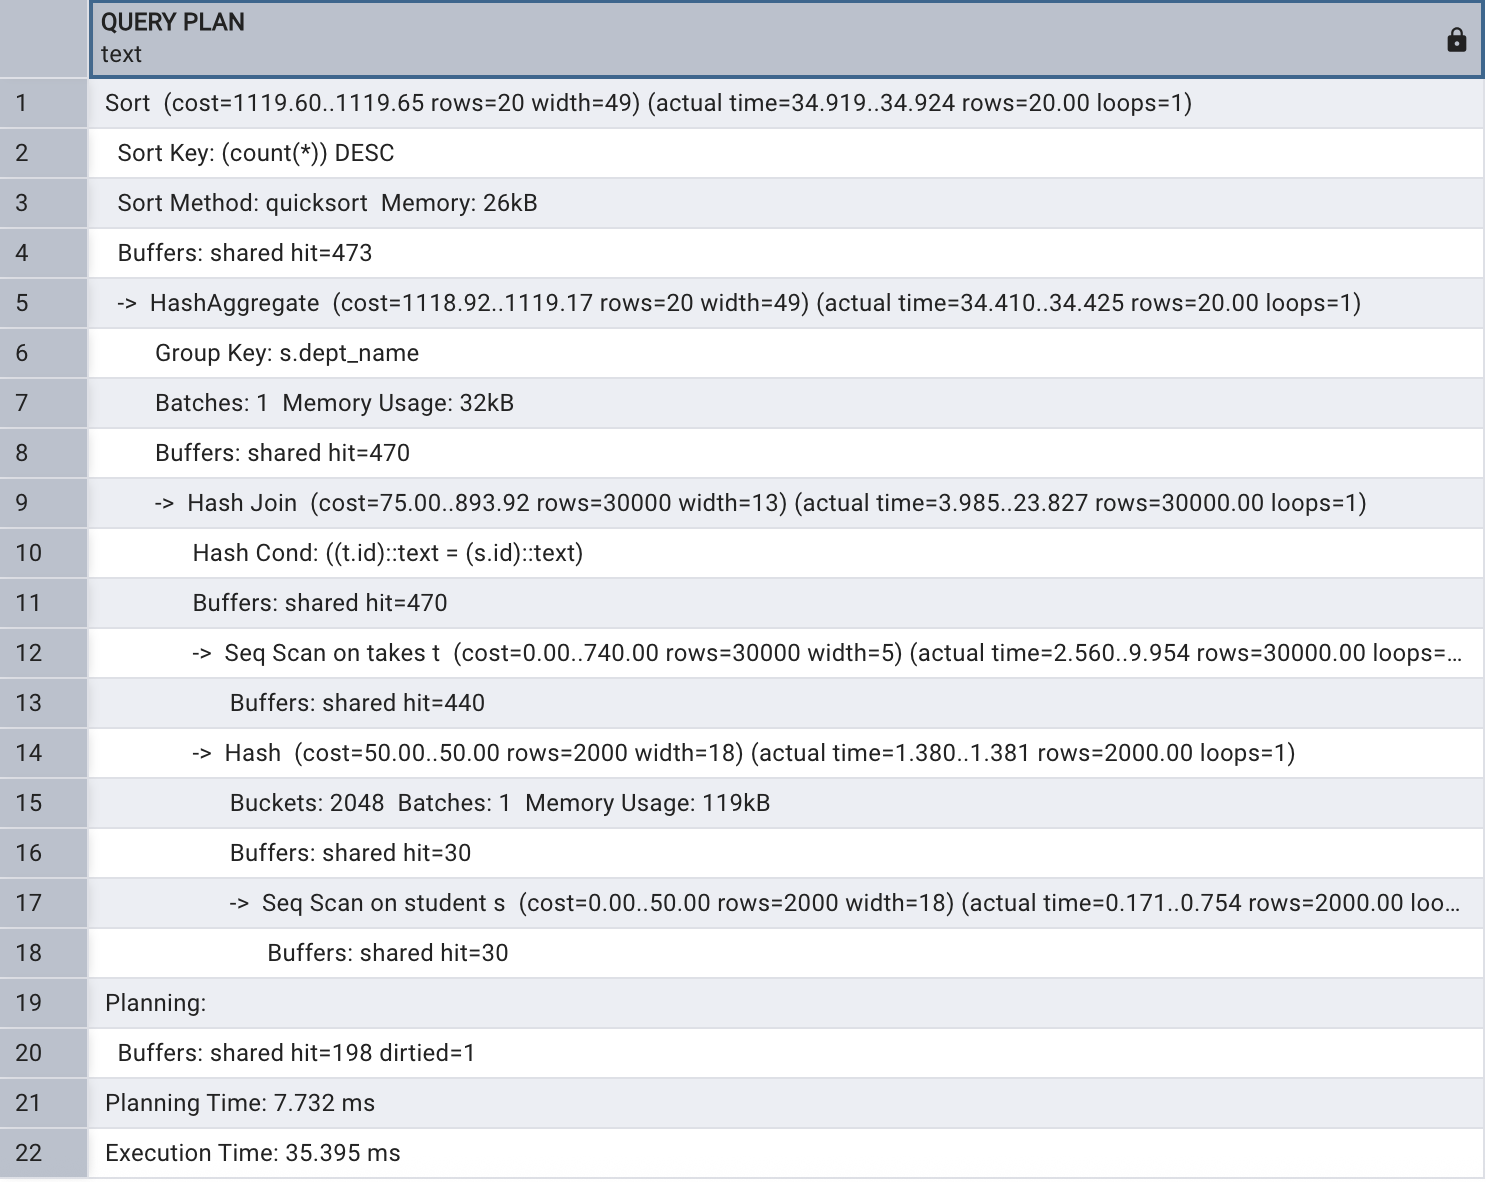
\includegraphics[keepaspectratio]{docs/images/Q1 explain.png}}

\paragraph{Performance/Correctness
Issue:}\label{performancecorrectness-issue}

\begin{enumerate}
\def\labelenumi{\arabic{enumi}.}
\tightlist
\item
  Joining student to takes: it changes the unit of analysis from
  averaging over students to averaging over enrollments, which is not
  what the prompt is asking
\item
  Sequential scan on takes: it unnecessarily scanned all 30,000 rows
  when it could have used a filter
\end{enumerate}

\subsubsection{\texorpdfstring{\textbf{Query 2 --- Multi-Table
Join}}{Query 2 --- Multi-Table Join}}\label{query-2-multi-table-join-1}

\paragraph{Execution Plan:}\label{execution-plan-1}

\pandocbounded{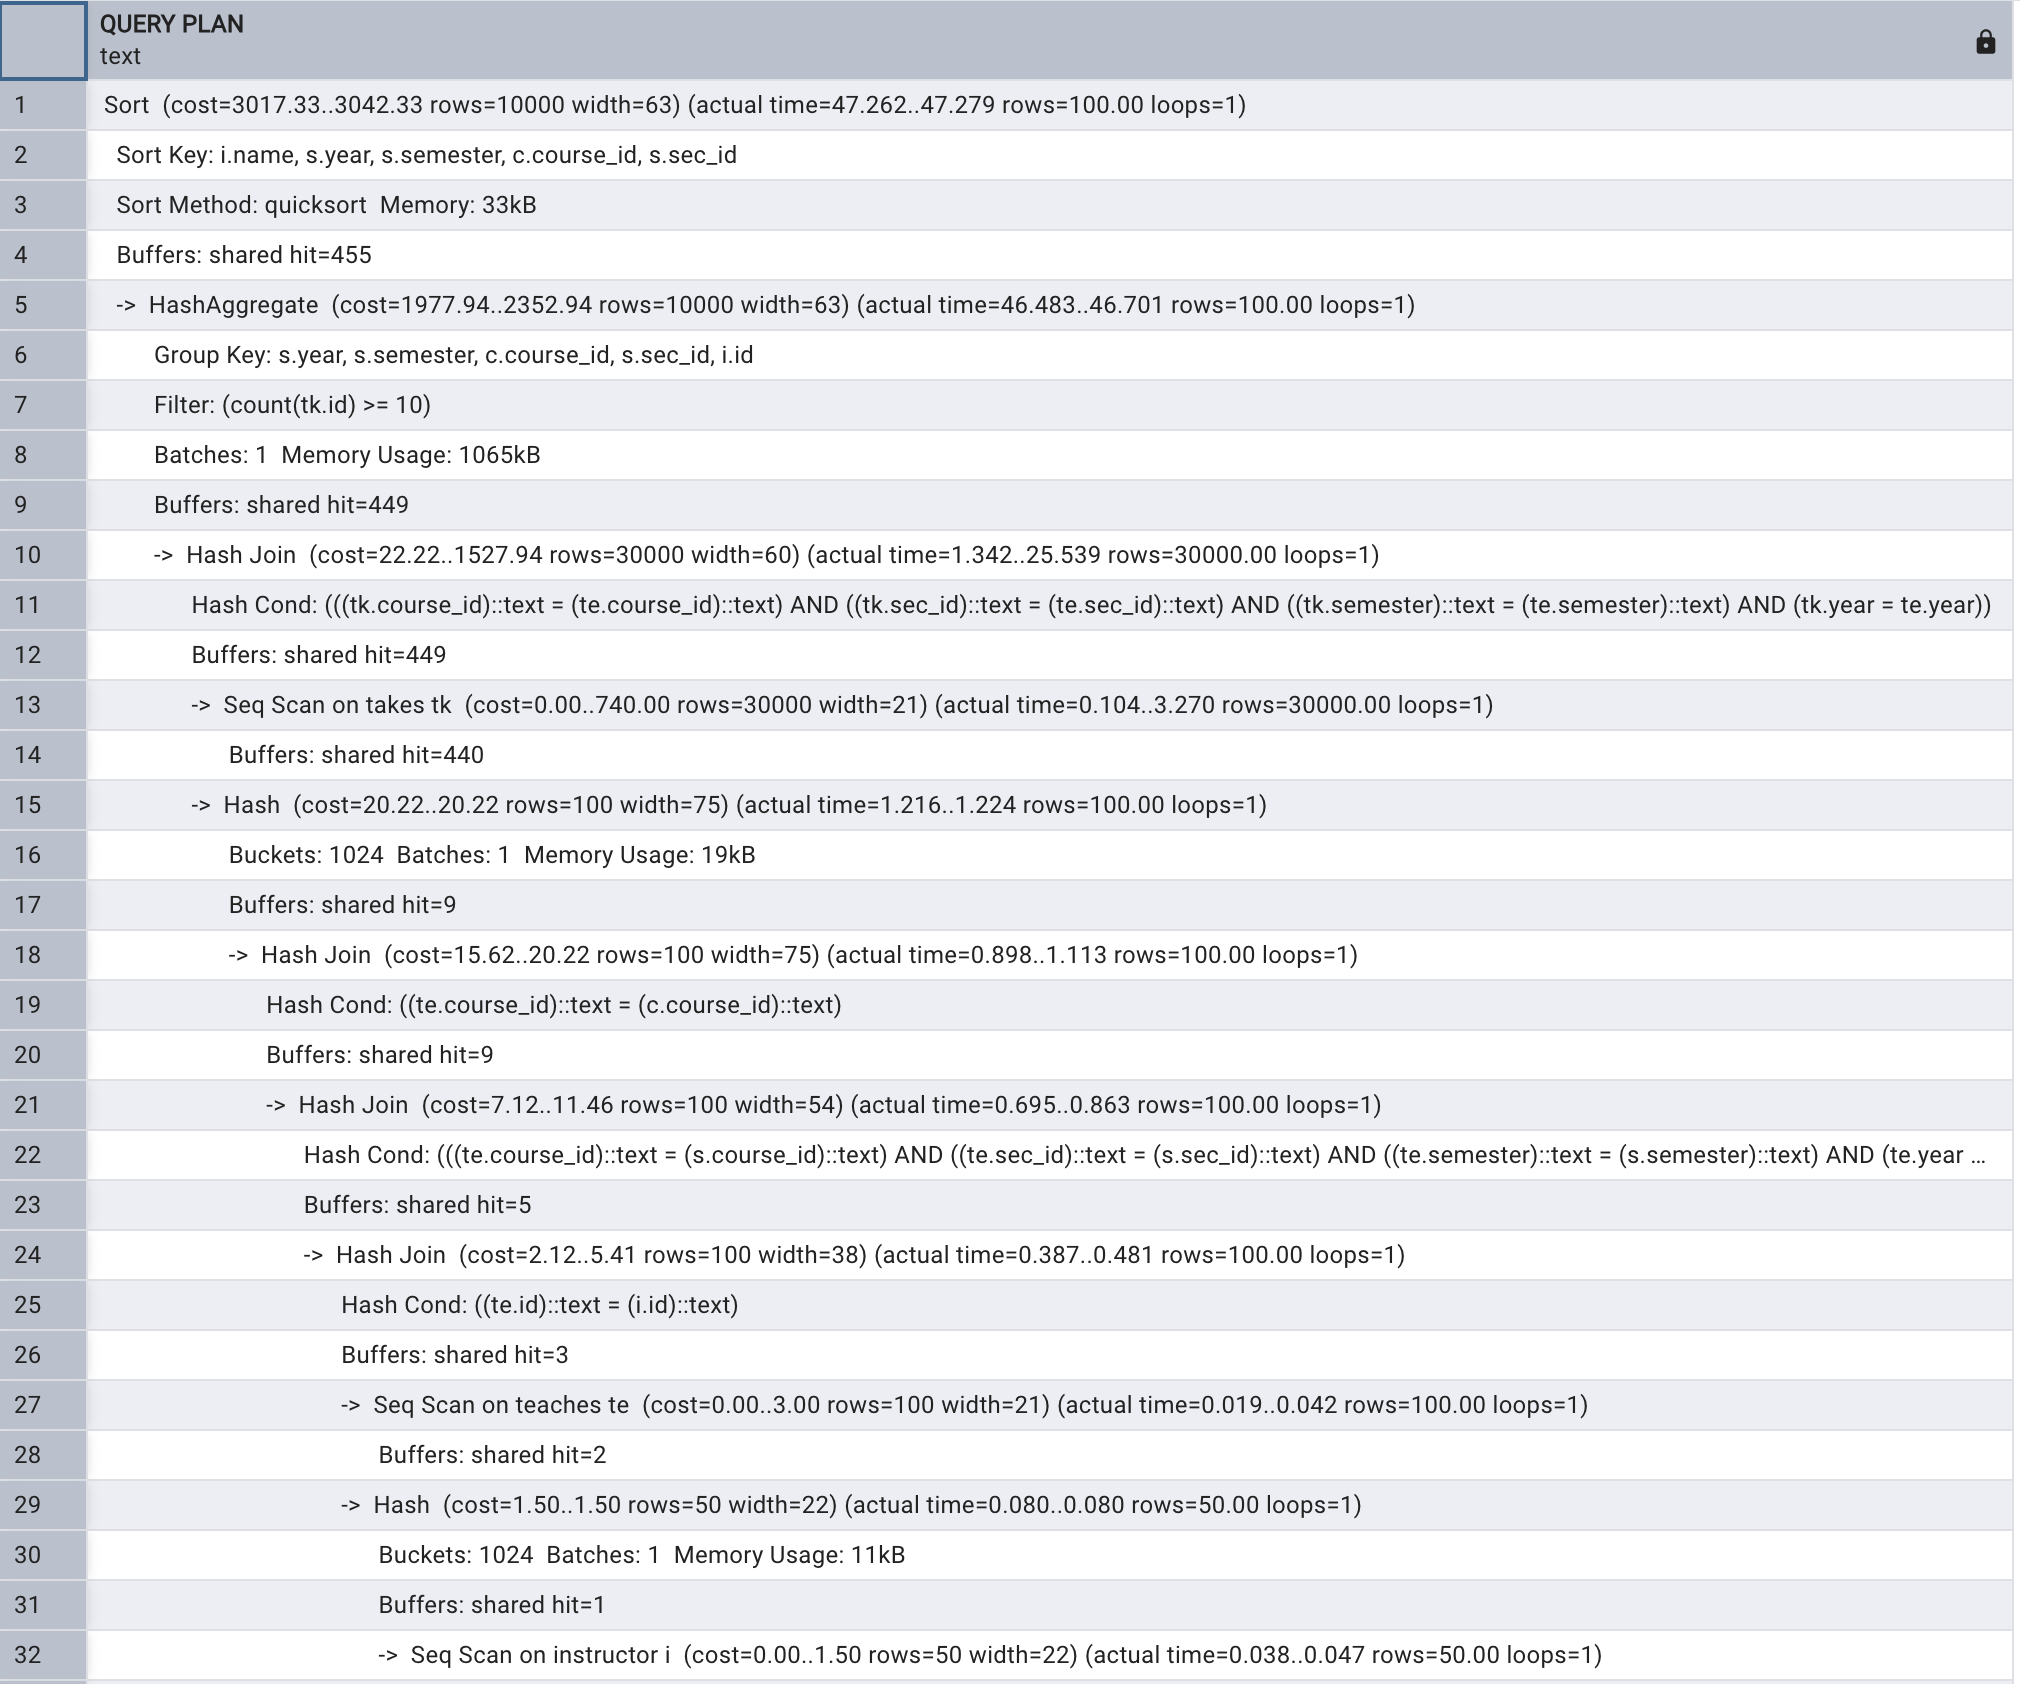
\includegraphics[keepaspectratio]{images/Q2 explain 1.png}}

\pandocbounded{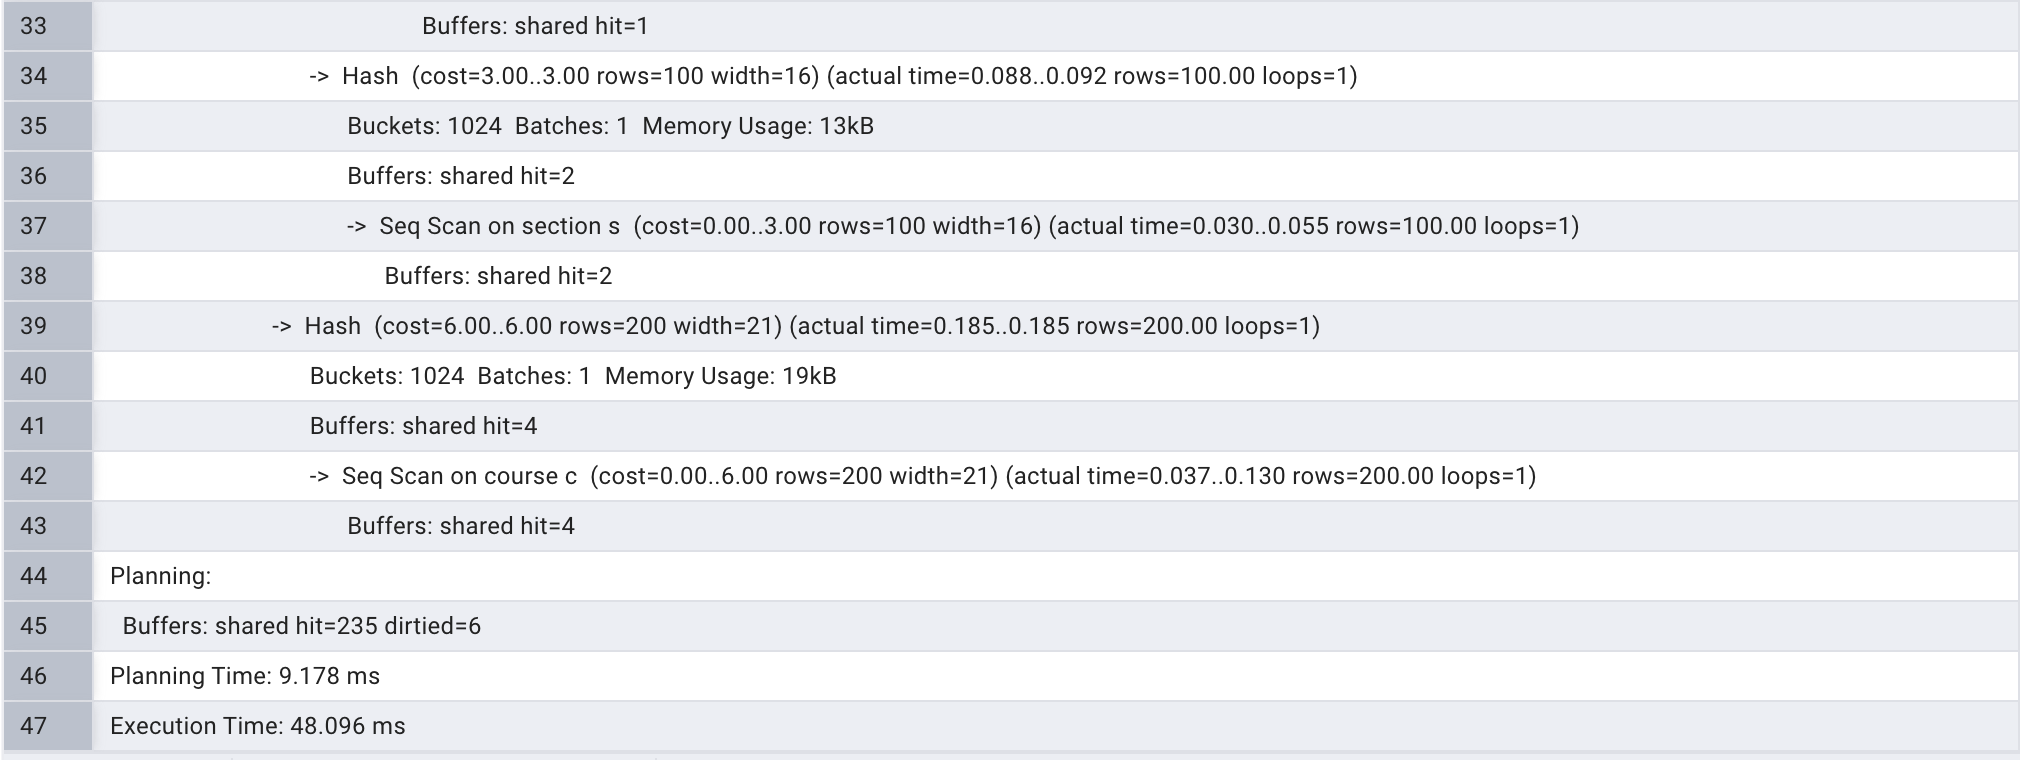
\includegraphics[keepaspectratio]{images/Q2 explain 2.png}}

\paragraph{Performance/Correctness
Issue:}\label{performancecorrectness-issue-1}

\begin{enumerate}
\def\labelenumi{\arabic{enumi}.}
\tightlist
\item
  Sequential scan on takes: it reads all 30,000 rows when it's
  unnecessary.
\item
  Sort Key: unnecessary order by at the end, can be replaced by Index
\end{enumerate}

\subsubsection{\texorpdfstring{\textbf{Query 3 ---} Correlated
Subquery}{Query 3 --- Correlated Subquery}}\label{query-3-correlated-subquery-1}

\paragraph{Execution Plan:}\label{execution-plan-2}

\pandocbounded{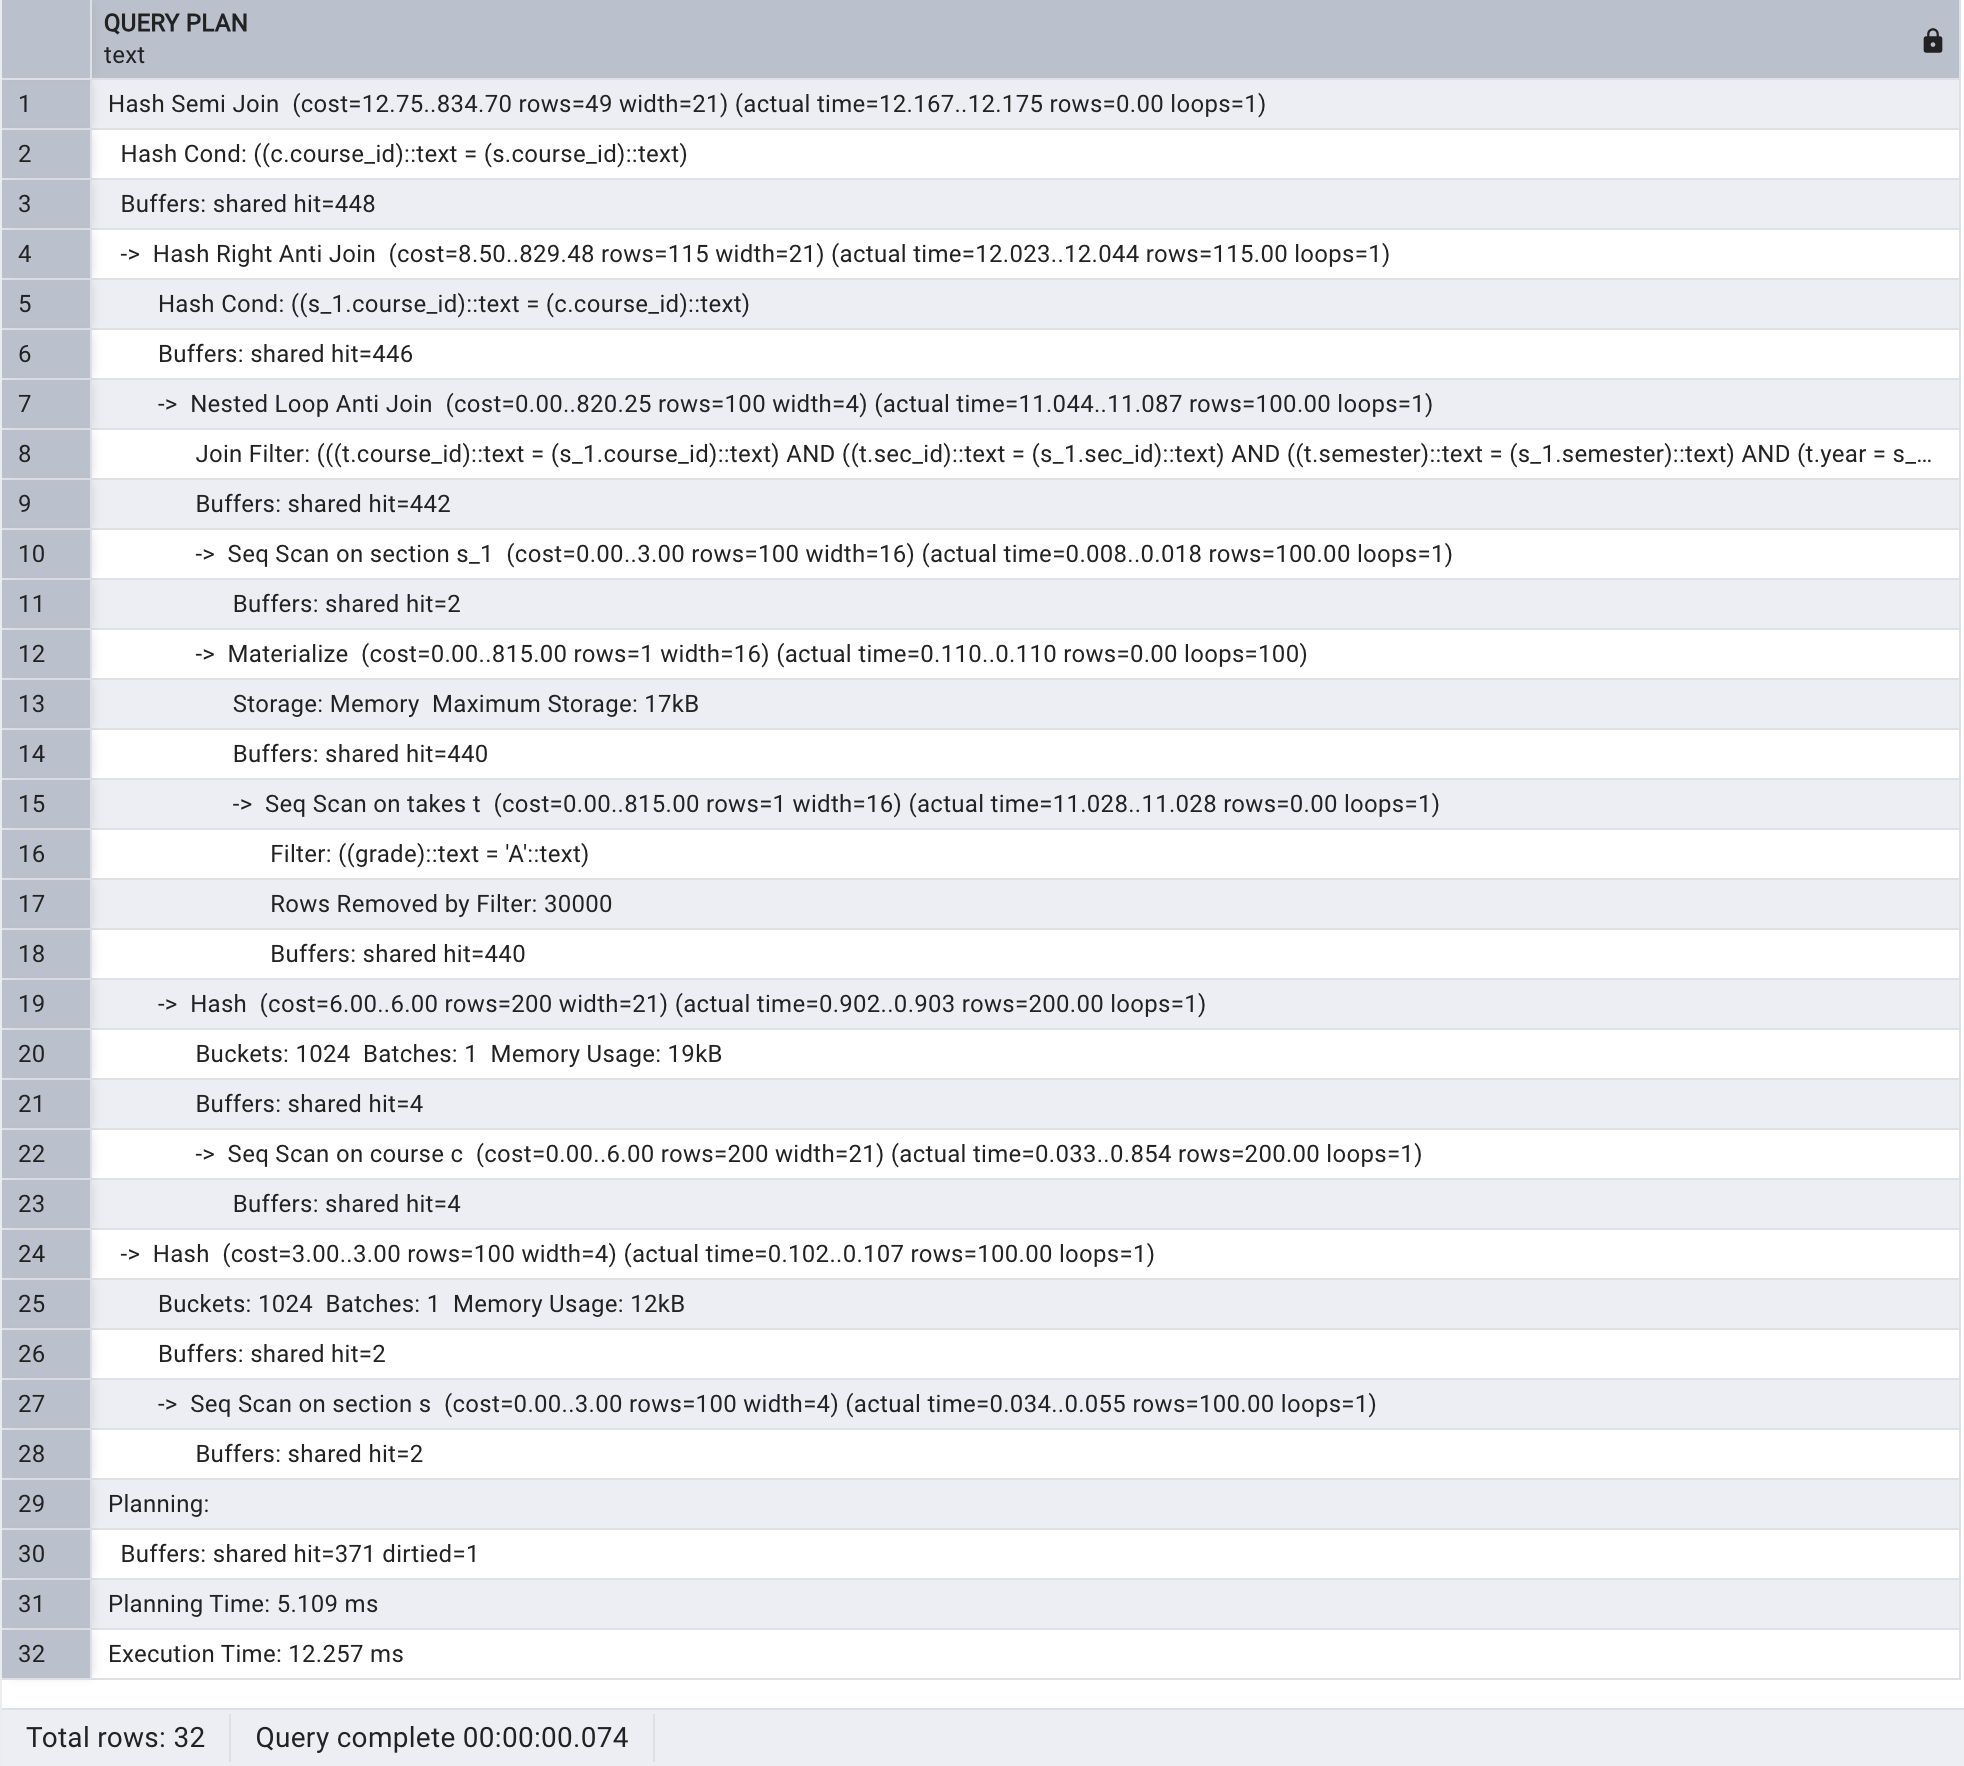
\includegraphics[keepaspectratio]{images/Q3 explain.png}}

\paragraph{Performance/Correctness
Issue:}\label{performancecorrectness-issue-2}

\begin{enumerate}
\def\labelenumi{\arabic{enumi}.}
\tightlist
\item
  Grade comparison: The AI SQL is filtering by `A' but it's not
  including `A+' or 'A-``, so it's returning 0 rows. This happens when
  AI doesn't know the data format.
\item
  Correlated subqueries: The plan included anti join logic (NOT EXIST,
  EXIST). Using HAVING instead is faster
\end{enumerate}

\subsubsection{\texorpdfstring{\textbf{Query 4 ---} Window
Function}{Query 4 --- Window Function}}\label{query-4-window-function-1}

\paragraph{Execution Plan:}\label{execution-plan-3}

\pandocbounded{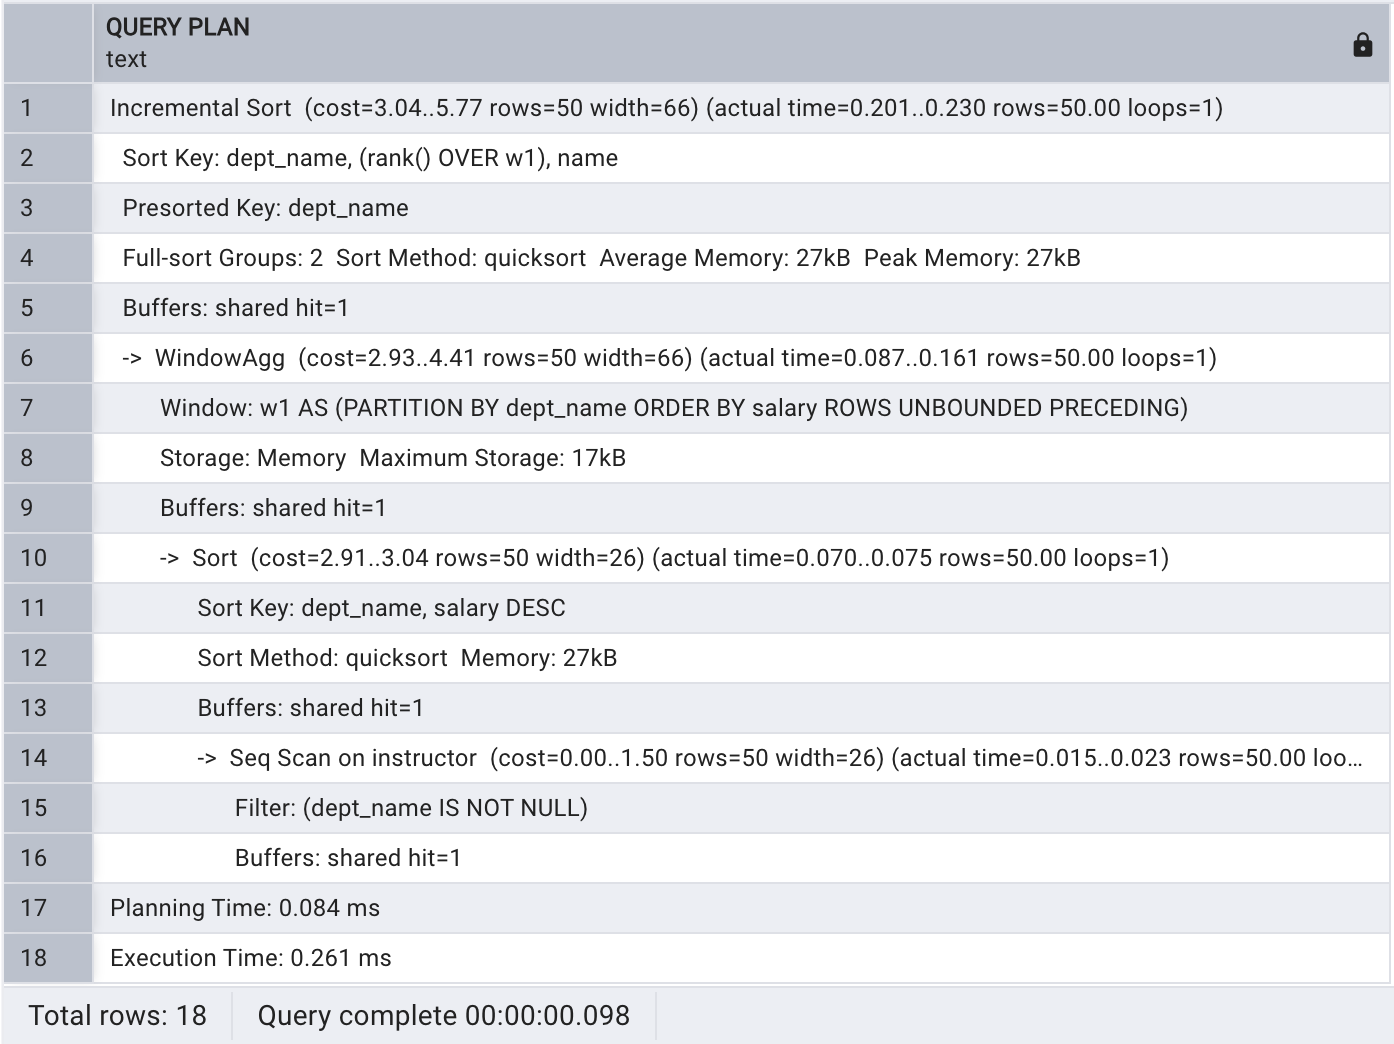
\includegraphics[keepaspectratio]{images/Q4 explain.png}}

\paragraph{Performance/Correctness
Issue:}\label{performancecorrectness-issue-3}

\begin{enumerate}
\def\labelenumi{\arabic{enumi}.}
\item
  Percentile logic: The query is using PERCENT\_RANK(), meaning that the
  highest paid instructor is given the rank of 0 and the lowest will get
  a rank of 1. This is backwards from what the prompt was asking, which
  was be percentile, not rank
\item
  Department NULL filter: The query includes the filter (dept\_name IS
  NOT NULL). It's unnecessary if the column is already non null by
  schema and could exclude rows if null departments were meant to be
  shown

  \subsubsection{\texorpdfstring{\textbf{Query 5 ---} Complex
  Query}{Query 5 --- Complex Query}}\label{query-5-complex-query-1}

  \paragraph{Execution Plan:}\label{execution-plan-4}

  \pandocbounded{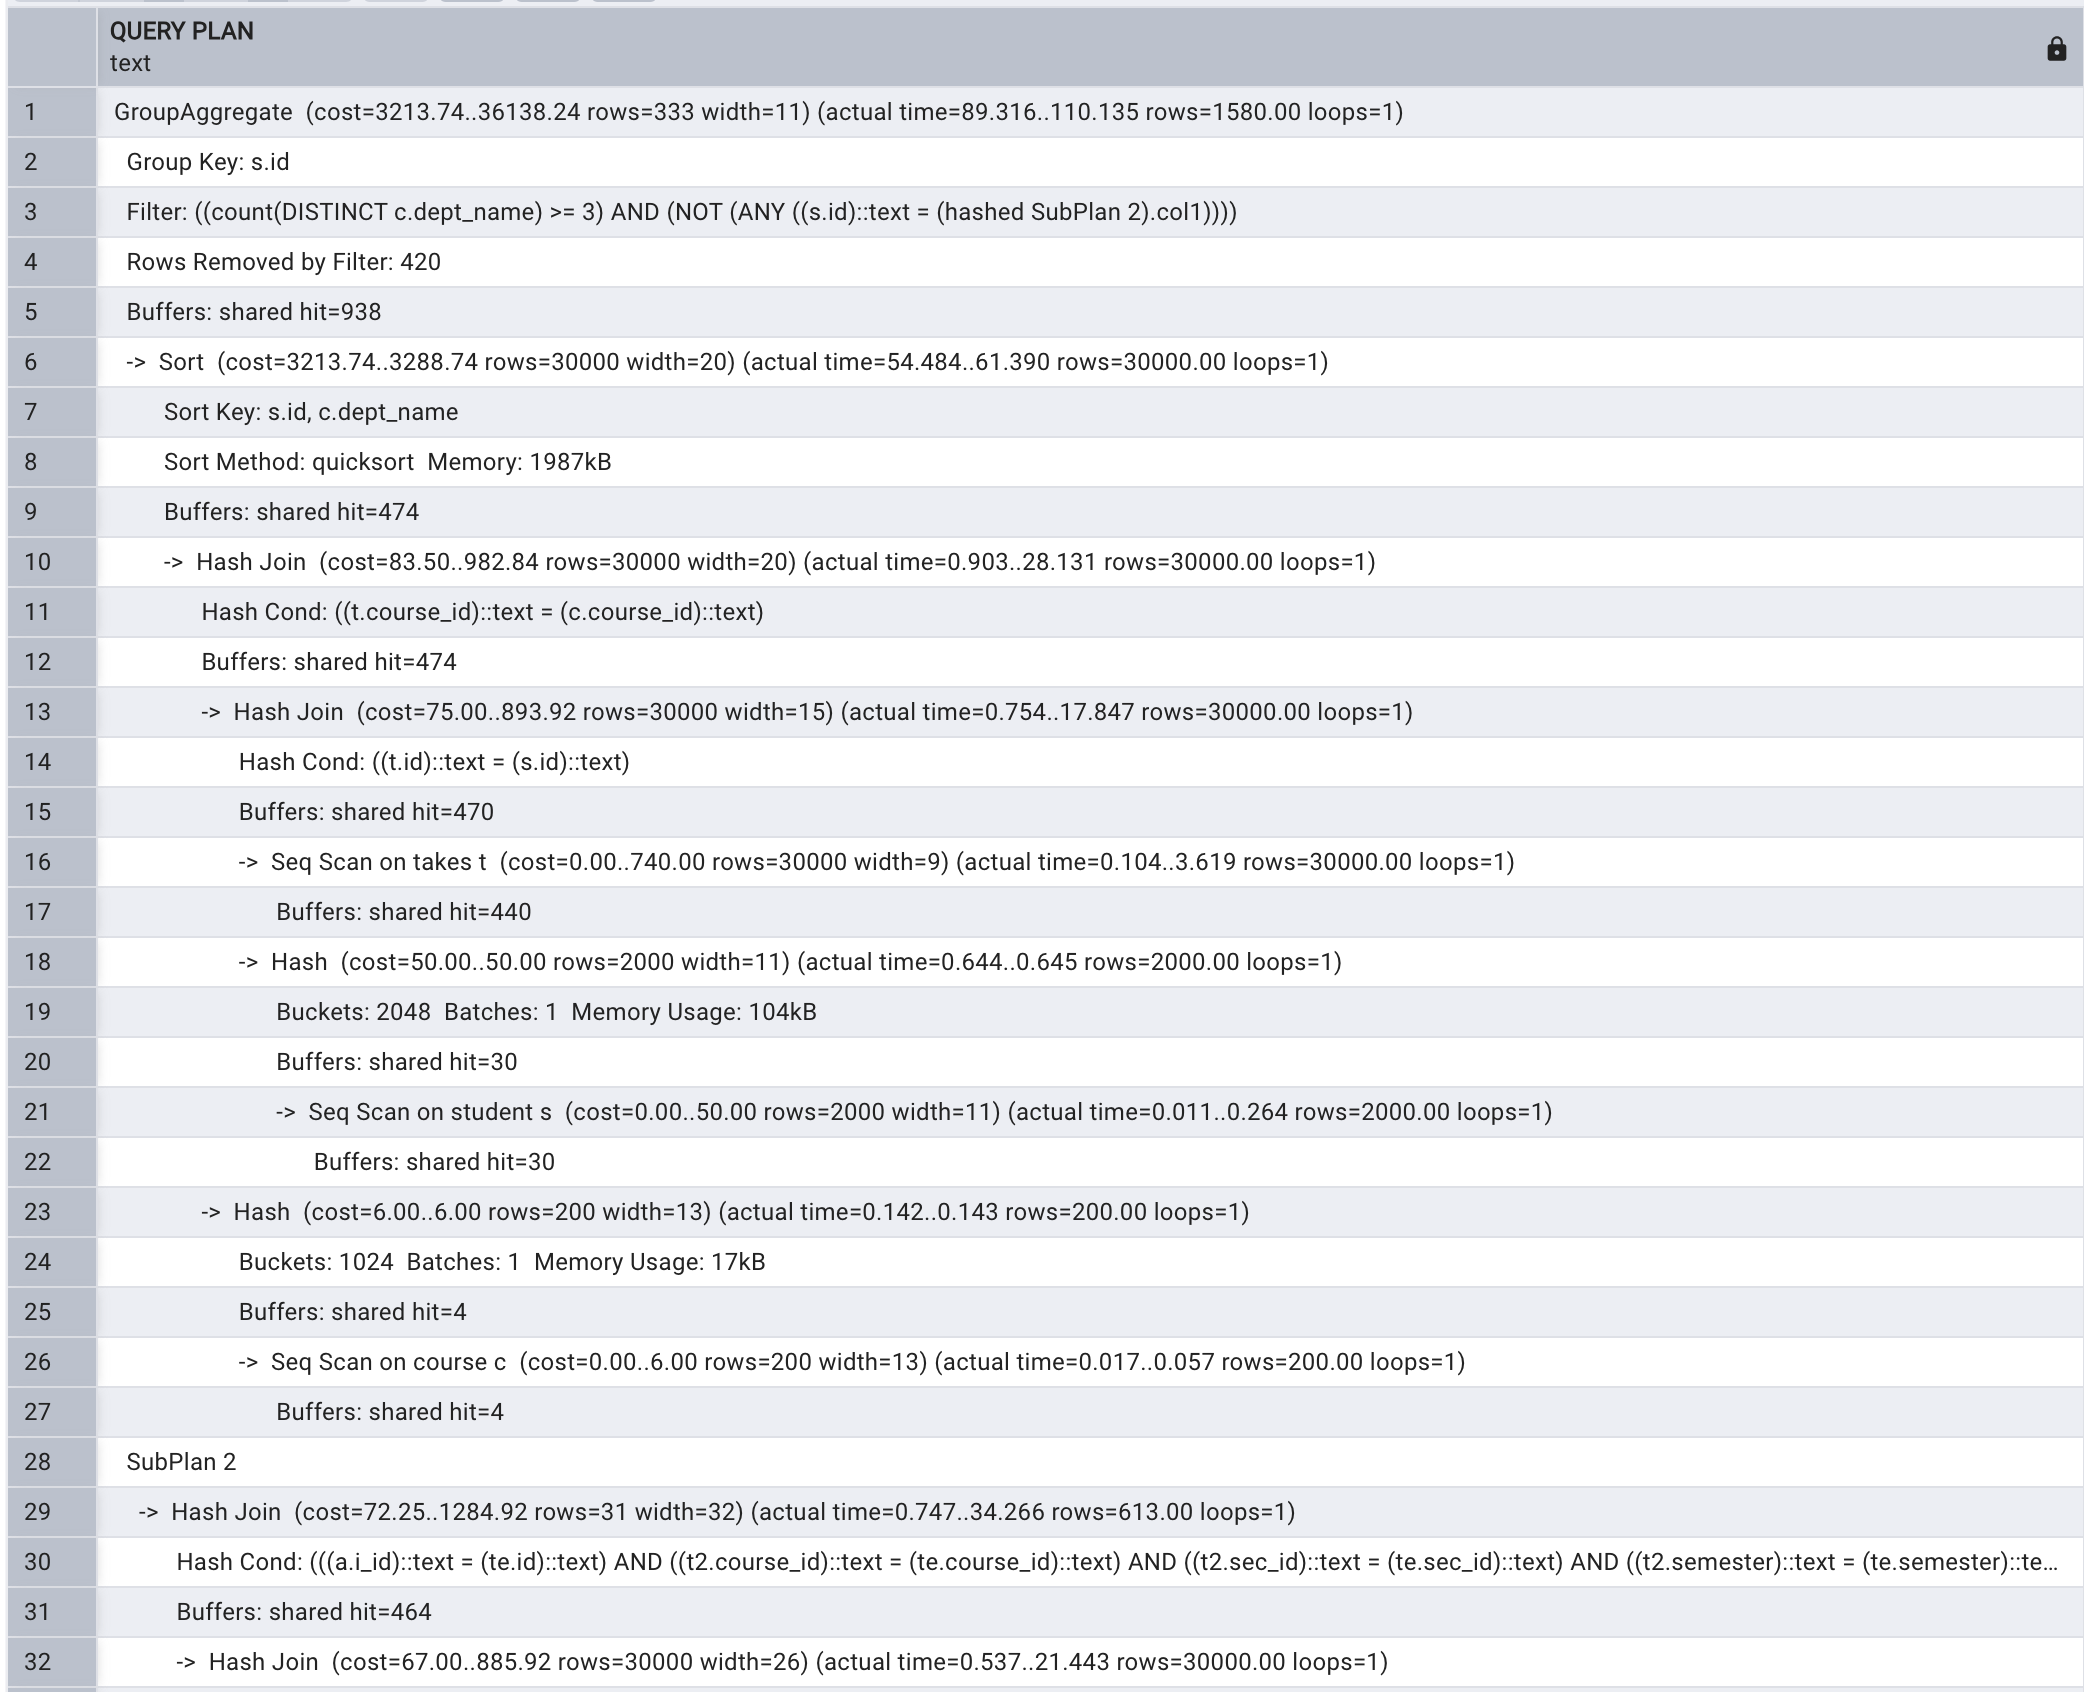
\includegraphics[keepaspectratio]{images/Q5 explain 1.png}}
\end{enumerate}

\pandocbounded{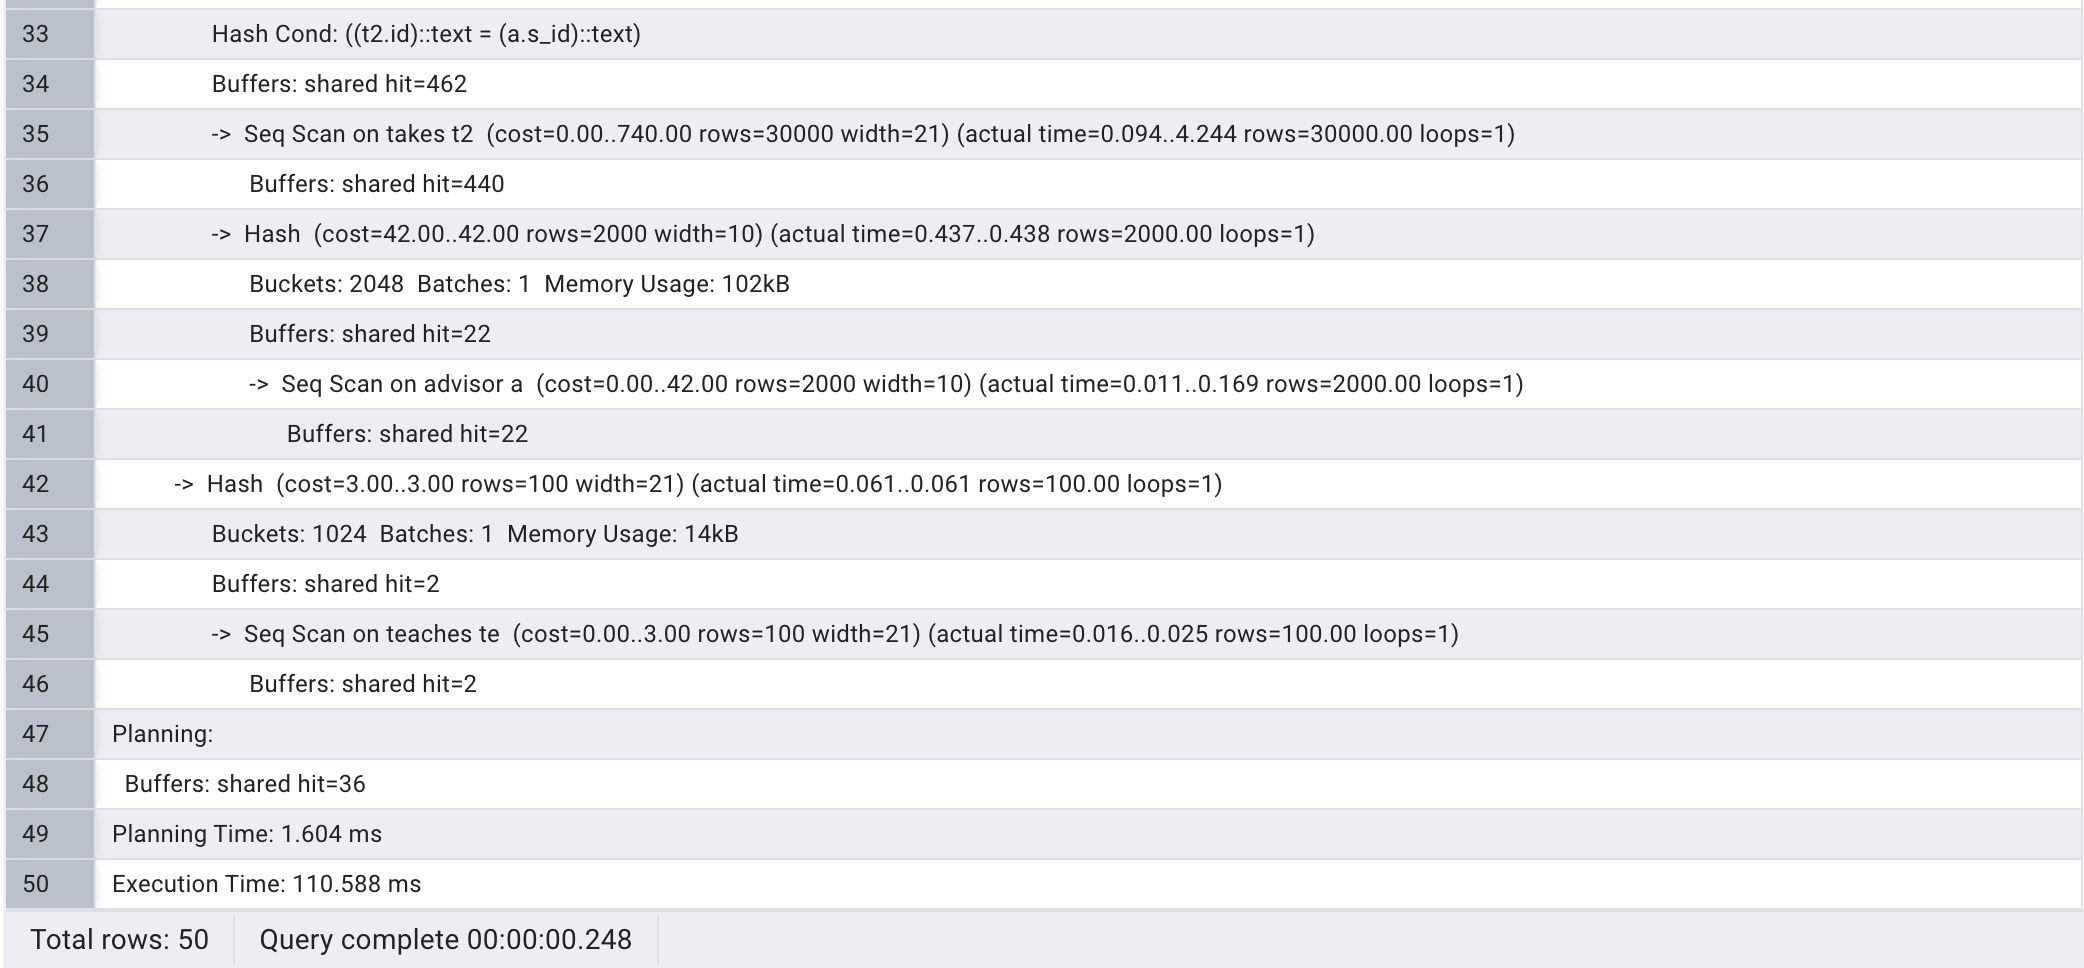
\includegraphics[keepaspectratio]{images/Q5 explain 2.png}}

\paragraph{Performance/Correctness
Issue:}\label{performancecorrectness-issue-4}

\begin{enumerate}
\def\labelenumi{\arabic{enumi}.}
\tightlist
\item
  Multiple sequential scan on takes: The query scans all 30,000 rows
  twice for `takes'. This can be consolidated by joining
\item
  Not exist: increases complexity and lads to multiple re scanning of
  `takes'.
\end{enumerate}

\subsection{Part 3: Query Optimization}\label{part-3-query-optimization}

\subsubsection{Query 1 --- Aggregation}\label{query-1-aggregation-2}

\paragraph{Indexes created}\label{indexes-created}

CREATE INDEX idx\_takes\_student\_id ON takes(ID);

CREATE INDEX idx\_course\_dept ON course(dept\_name);

\paragraph{Optimized Version}\label{optimized-version}

\begin{verbatim}
\end{verbatim}

\paragraph{New Execution Plan}\label{new-execution-plan}

\paragraph{Performance Comparison}\label{performance-comparison}

\begin{longtable}[]{@{}llll@{}}
\toprule\noalign{}
Metric & Before & After & Change \\
\midrule\noalign{}
\endhead
\bottomrule\noalign{}
\endlastfoot
Scan type on takes & seq scan & index scan & \\
Join students to take & avg(s.tot\_cred) & use CTE & \\
Rows scanned & 30000 & 30000 & 0\% \\
Execution Tim & 274 & 92 & -66\% \\
\end{longtable}

\subsubsection{\texorpdfstring{\textbf{Query 2 --- Multi-Table
Join}}{Query 2 --- Multi-Table Join}}\label{query-2-multi-table-join-2}

\paragraph{Indexes created}\label{indexes-created-1}

CREATE INDEX idx\_takes\_student\_id ON takes(ID)

CREATE INDEX idx\_takes\_section

ON takes(course\_id, sec\_id, semester, year);

\paragraph{Optimized Version}\label{optimized-version-1}

\begin{verbatim}
SELECT
    i.name AS instructor_name,
    i.dept_name AS instructor_department,
    c.course_id,
    c.title AS course_title,
    s.sec_id,
    s.semester,
    s.year,
    COUNT(tk.ID) AS enrolled_students
FROM instructor AS i
JOIN teaches AS te
    ON i.ID = te.ID
JOIN section AS s
    ON te.course_id = s.course_id
   AND te.sec_id = s.sec_id
   AND te.semester = s.semester
   AND te.year = s.year
JOIN course AS c
    ON s.course_id = c.course_id
JOIN takes AS tk
    ON s.course_id = tk.course_id
   AND s.sec_id = tk.sec_id
   AND s.semester = tk.semester
   AND s.year = tk.year
GROUP BY
    i.ID,
    i.name,
    i.dept_name,
    c.course_id,
    c.title,
    s.sec_id,
    s.semester,
    s.year
HAVING COUNT(tk.ID) >= 10
ORDER BY i.dept_name DESC, i.name;
\end{verbatim}

\paragraph{New Execution Plan}\label{new-execution-plan-1}

\pandocbounded{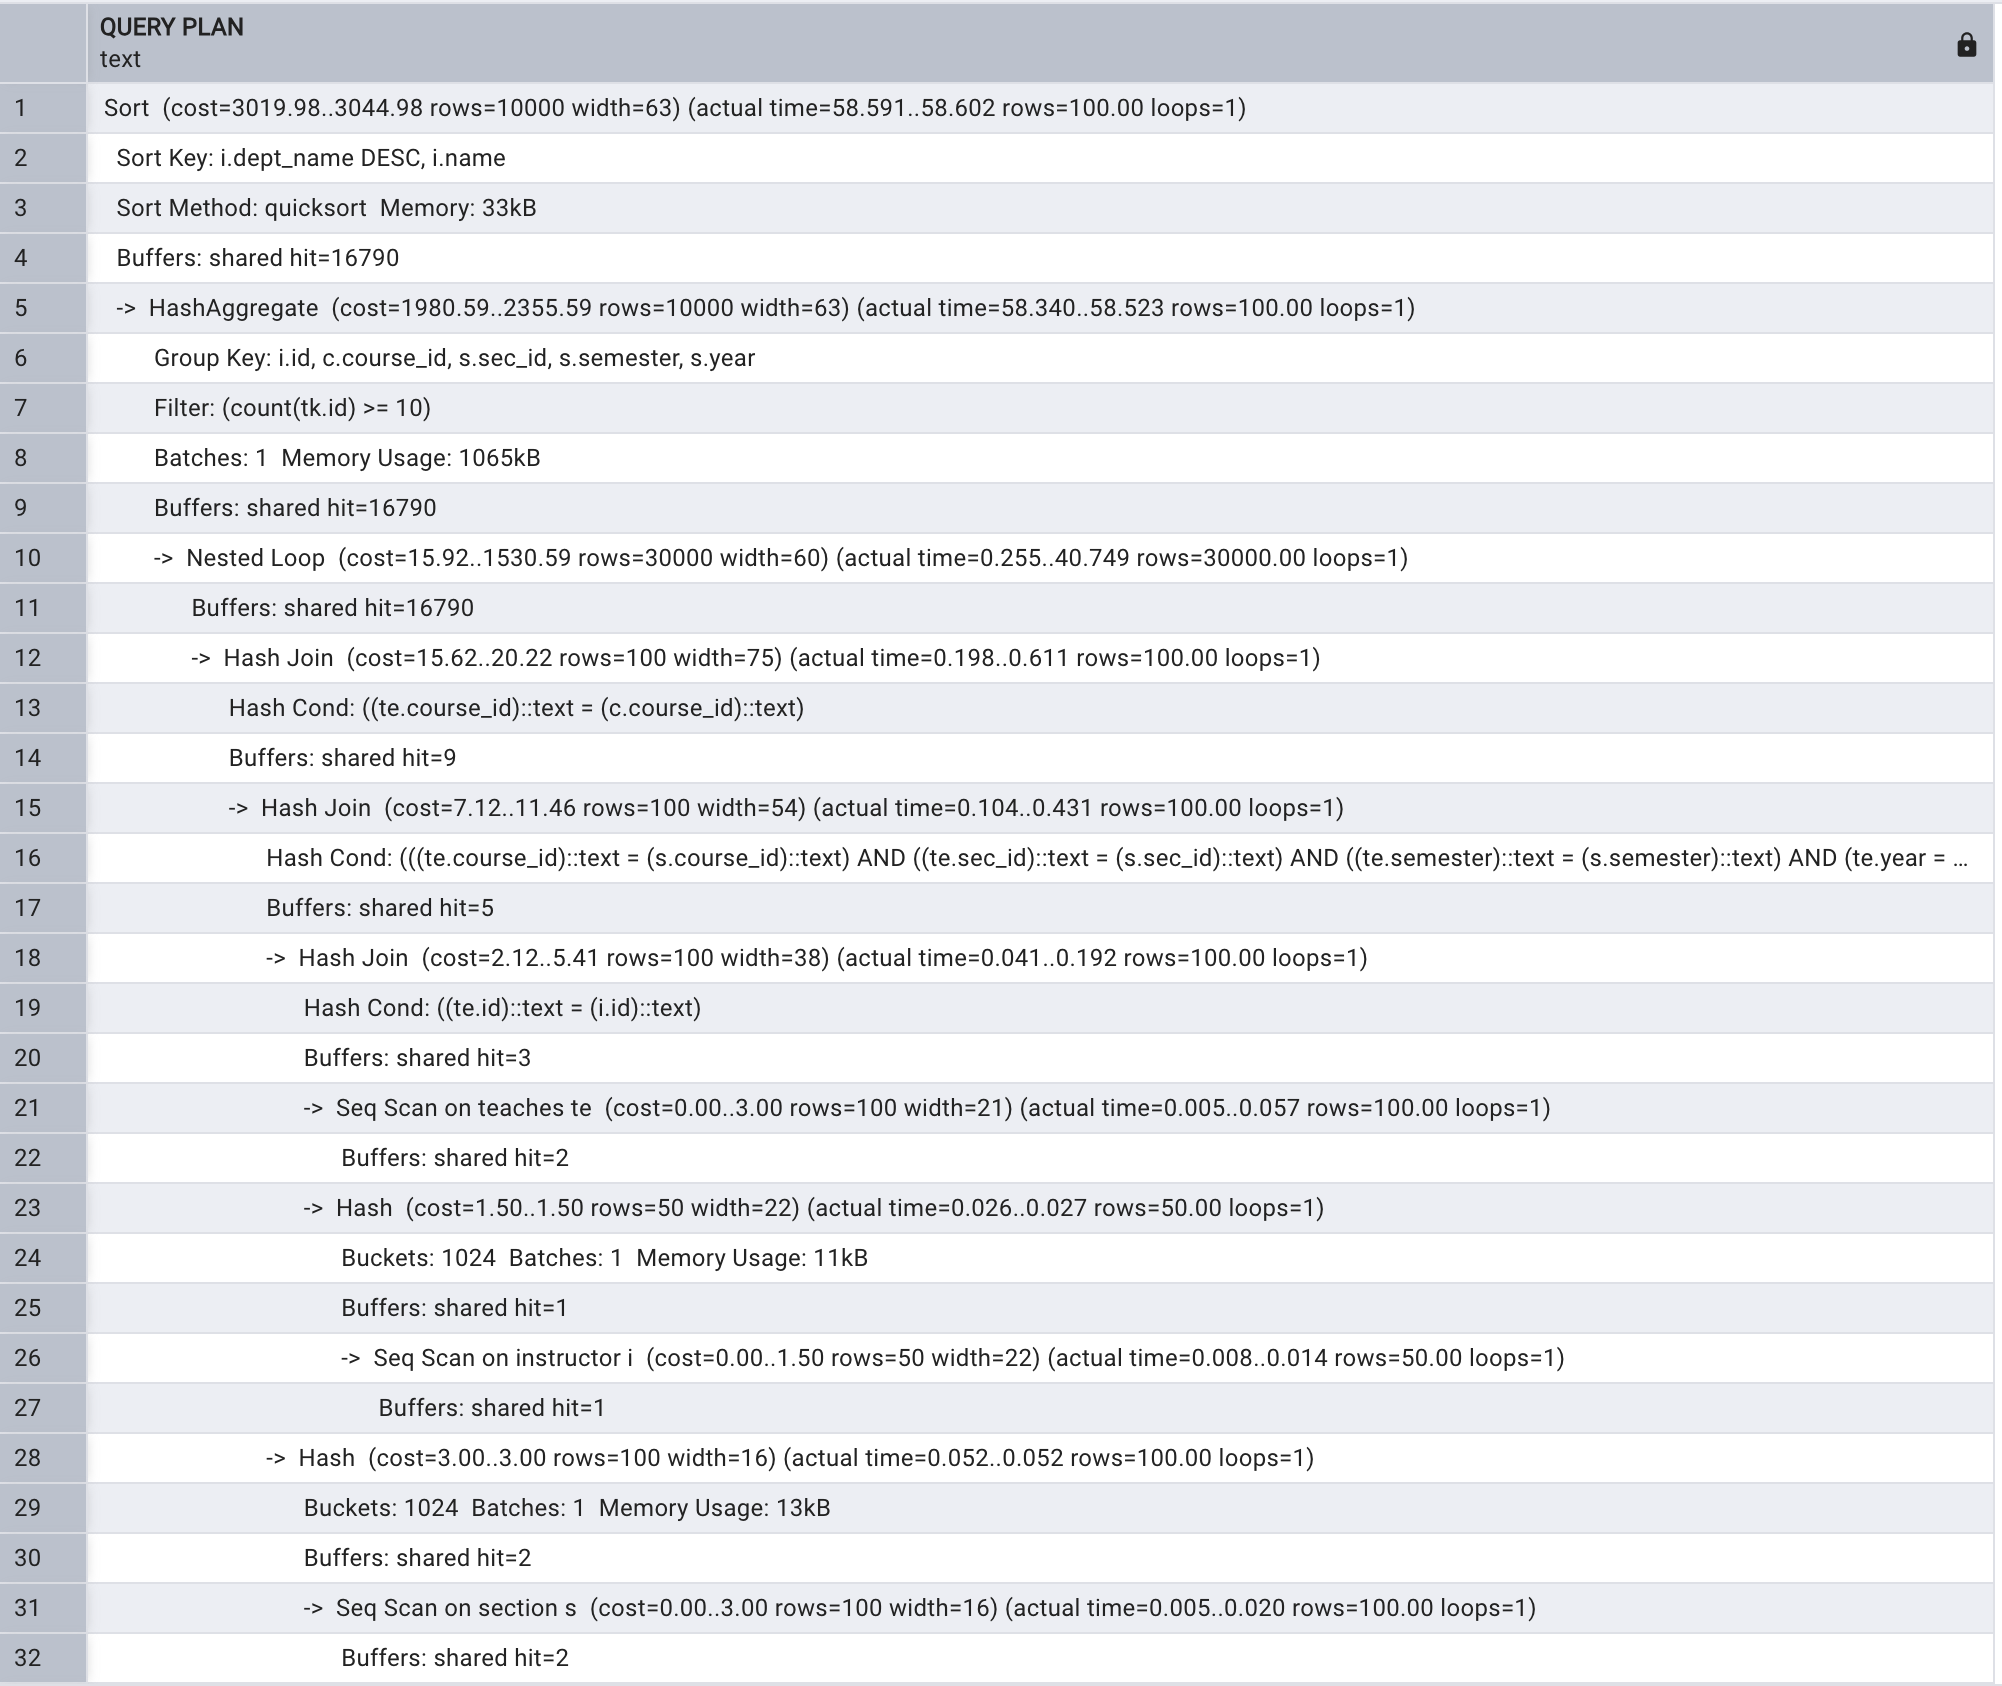
\includegraphics[keepaspectratio]{images/NEW Q2 explain 1.png}}

\pandocbounded{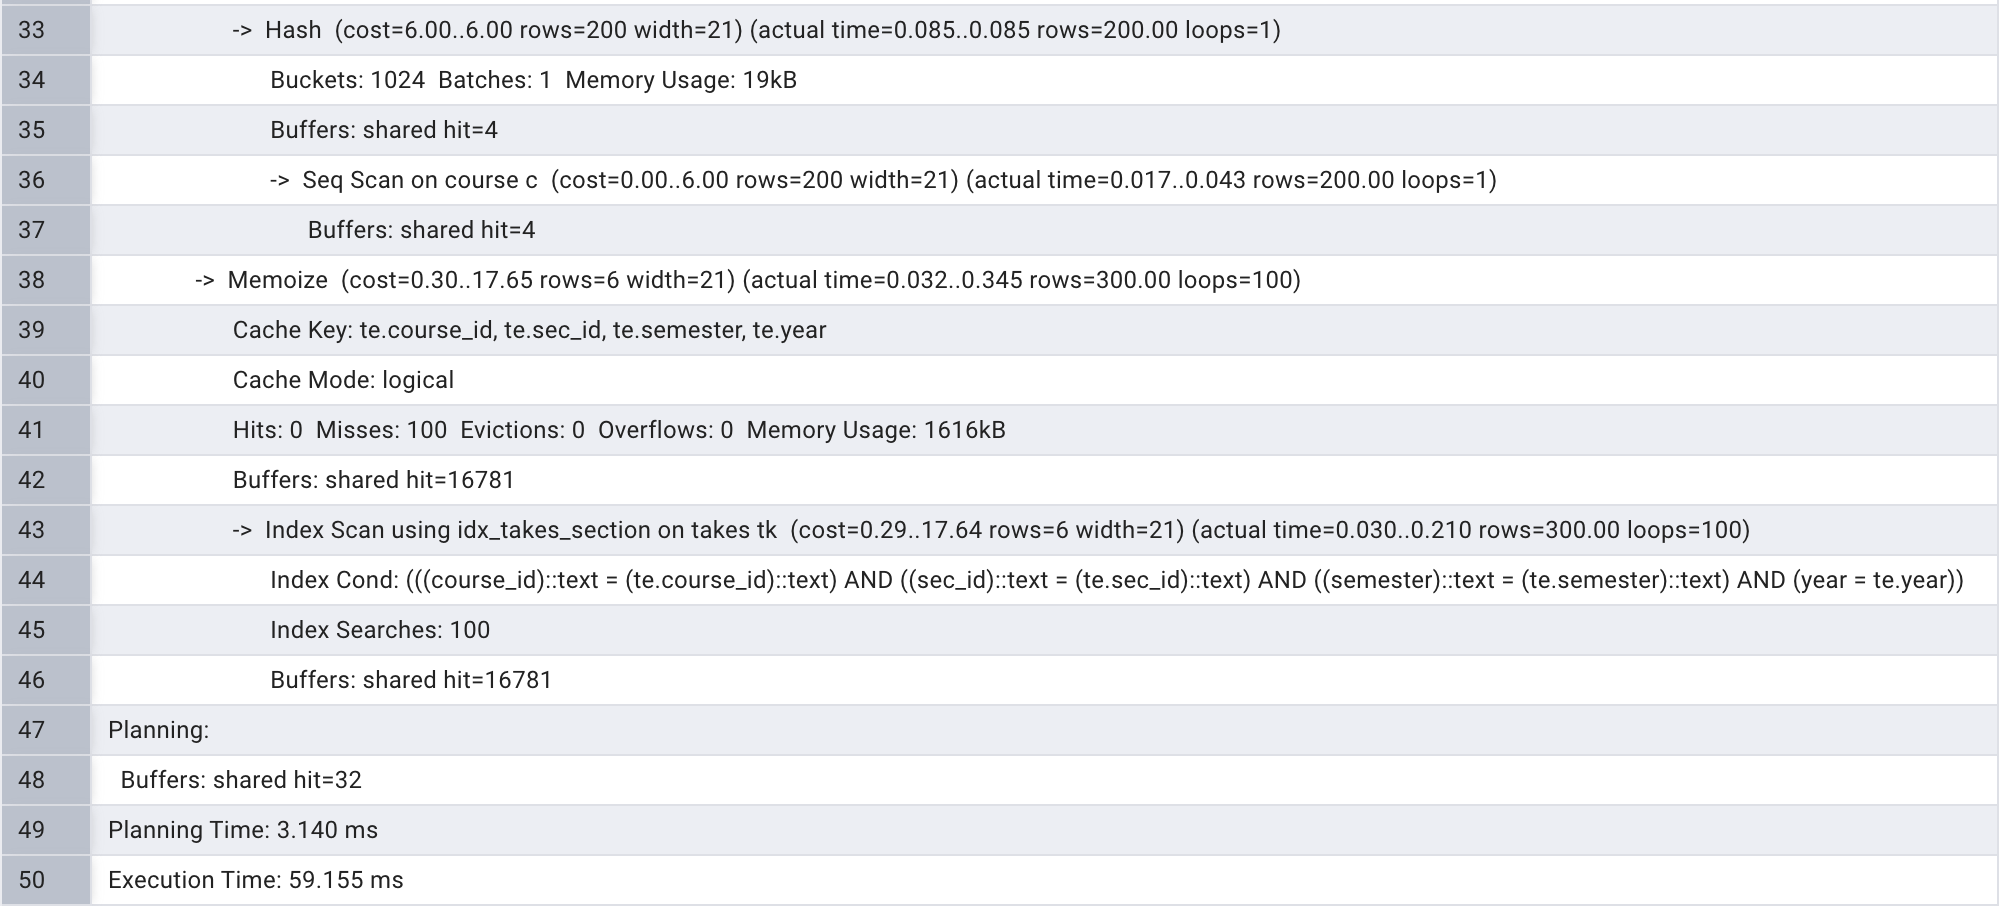
\includegraphics[keepaspectratio]{images/New Q2 explain 2.png}}

\paragraph{Performance Comparison}\label{performance-comparison-1}

\begin{longtable}[]{@{}llll@{}}
\toprule\noalign{}
Metric & Before & After & Change \\
\midrule\noalign{}
\endhead
\bottomrule\noalign{}
\endlastfoot
Scan type on takes & Seq scan & Index Scan & \\
Rows scanned & 30,000 & 300 & -99\% \\
Execution Time & 173ms & 59ms & -65.9 \\
\end{longtable}

\subsubsection{\texorpdfstring{\textbf{Query 3 ---} Correlated
Subquery}{Query 3 --- Correlated Subquery}}\label{query-3-correlated-subquery-2}

\paragraph{Indexes created}\label{indexes-created-2}

CREATE INDEX idx\_takes\_grade\_covering

ON takes(course\_id, sec\_id, semester, year)

INCLUDE (ID, grade);

\paragraph{Optimized Version}\label{optimized-version-2}

\begin{verbatim}
SELECT c.course_id, c.title
FROM course c
JOIN section sec ON c.course_id = sec.course_id
LEFT JOIN takes t ON sec.course_id = t.course_id
AND sec.sec_id = t.sec_id
AND sec.semester = t.semester
AND sec.year = t.year
AND t.grade LIKE 'A%'
GROUP BY c.course_id, c.title
HAVING COUNT(DISTINCT sec.course_id || sec.sec_id || sec.semester || sec.year)
= COUNT(DISTINCT CASE WHEN t.grade LIKE 'A%'
THEN sec.course_id || sec.sec_id || sec.semester || sec.year
END);
\end{verbatim}

\paragraph{New Execution Plan}\label{new-execution-plan-2}

\pandocbounded{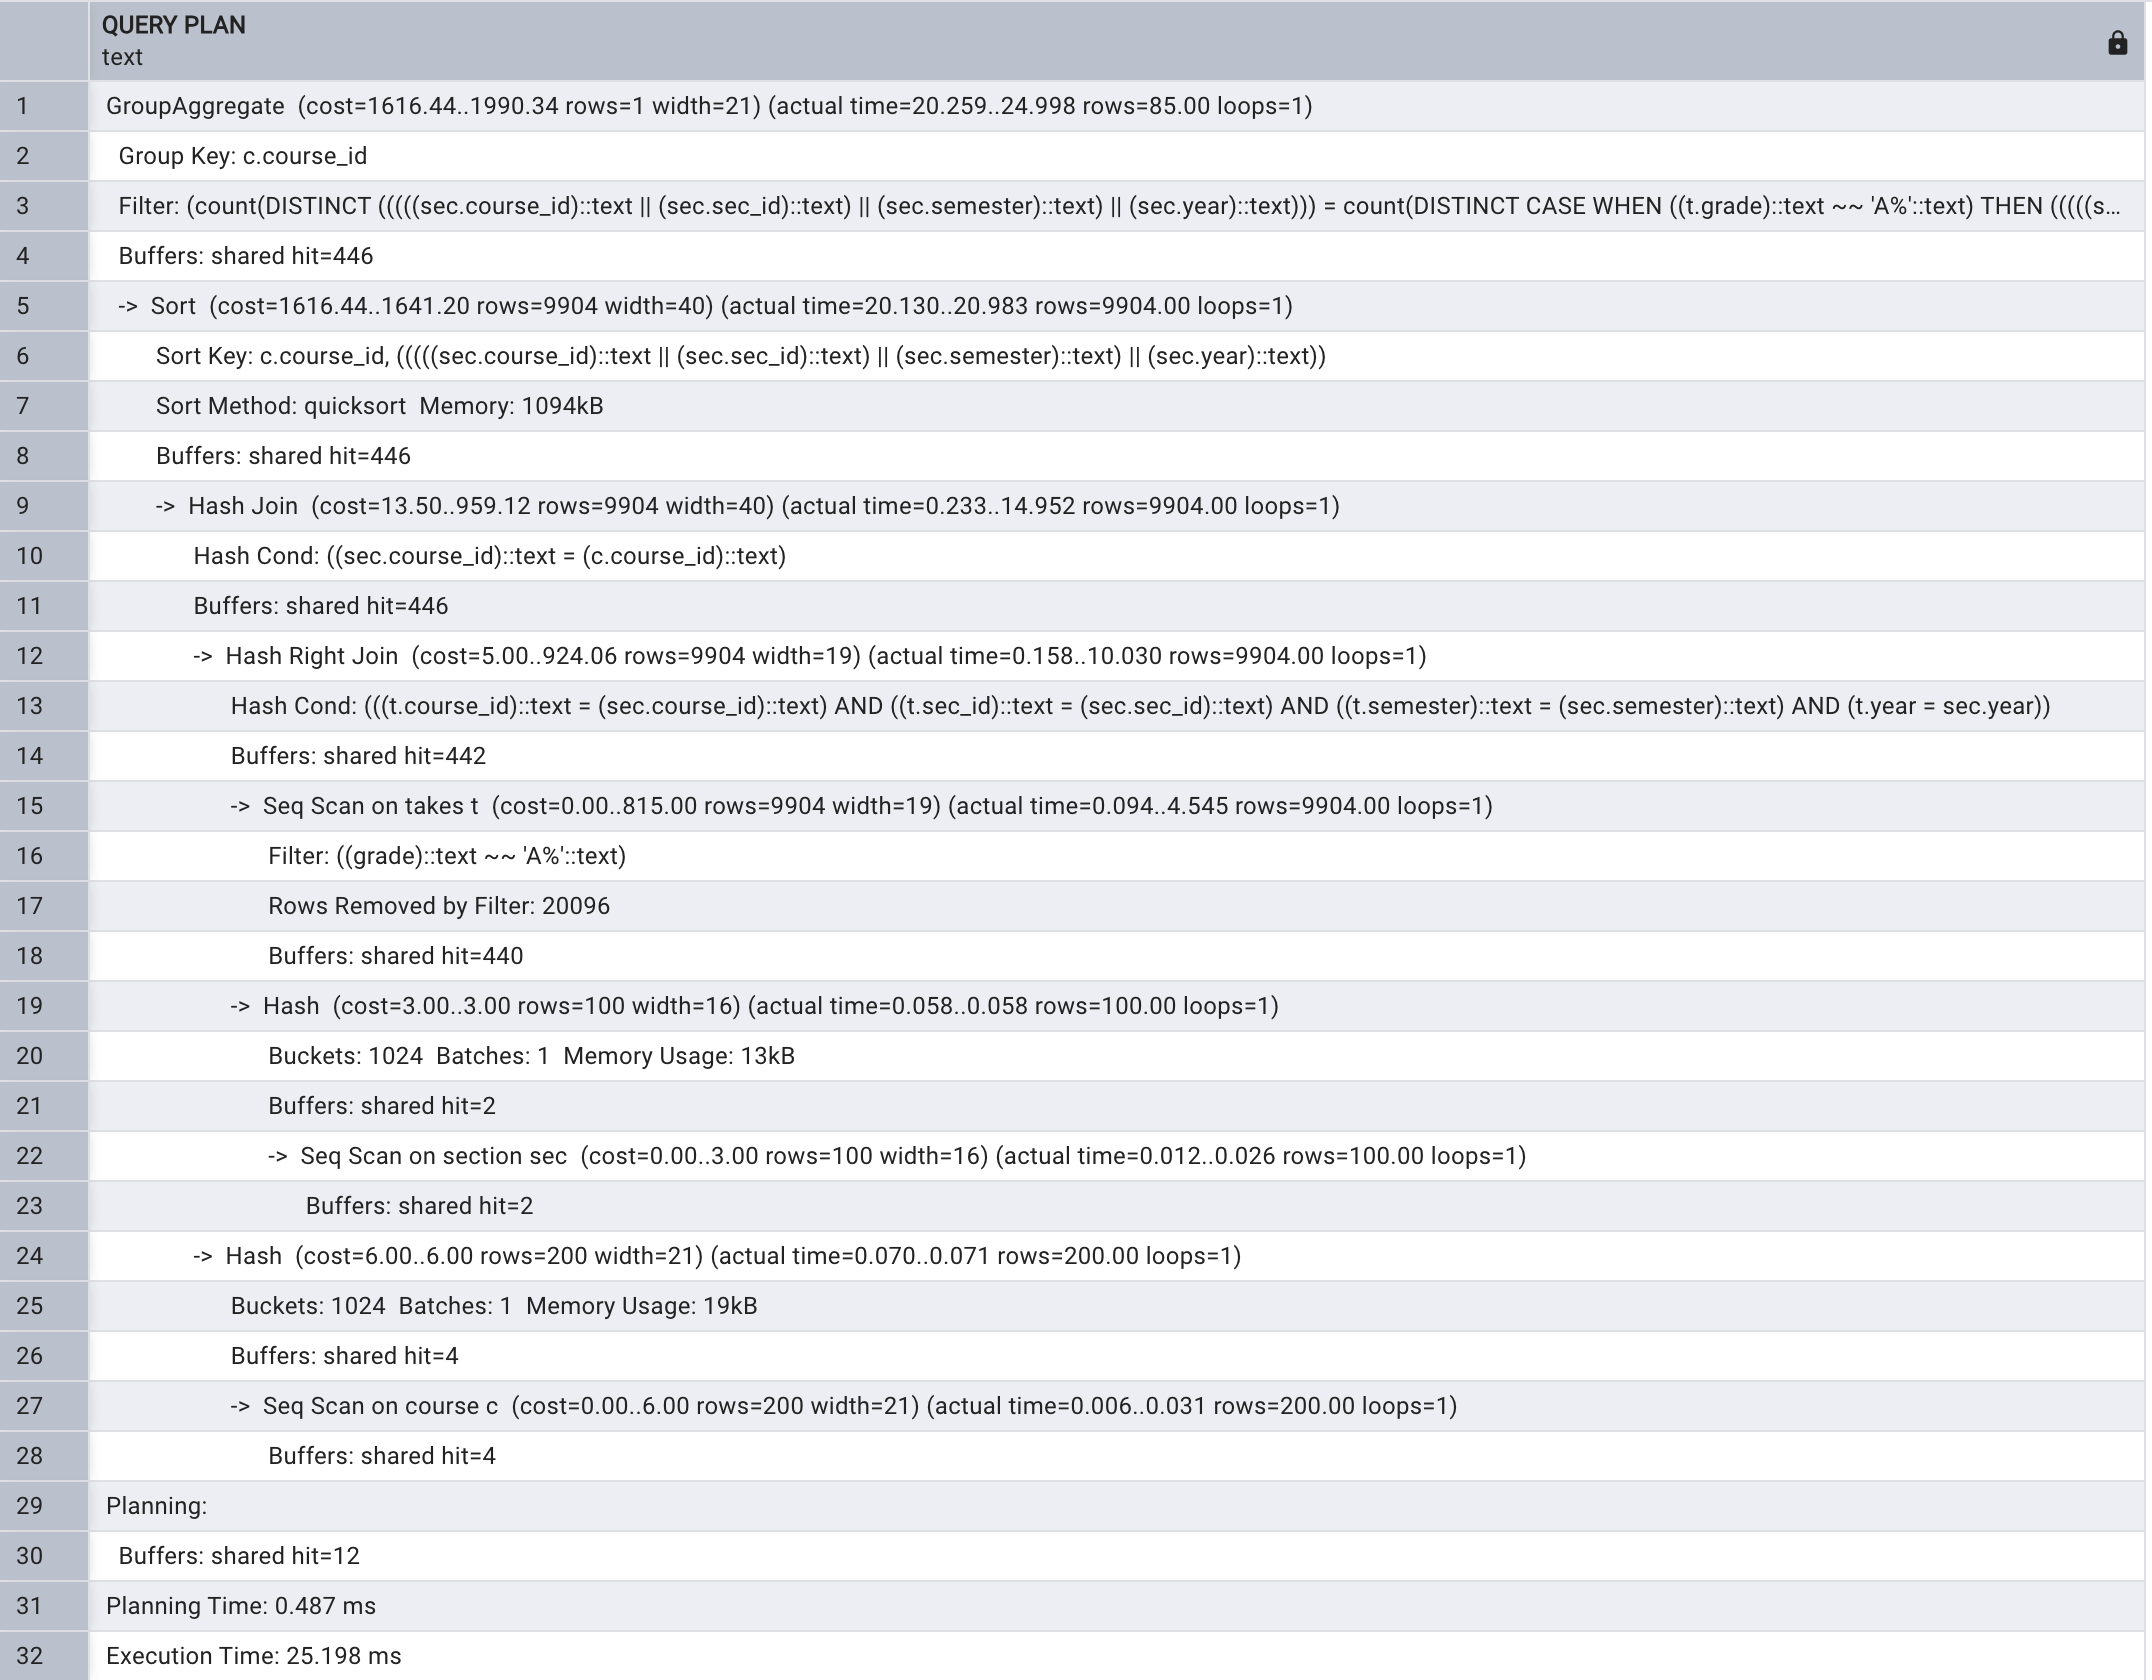
\includegraphics[keepaspectratio]{images/NEW Q3 explain.png}}

\paragraph{Performance Comparison}\label{performance-comparison-2}

\begin{longtable}[]{@{}llll@{}}
\toprule\noalign{}
Metric & Before & After & Change \\
\midrule\noalign{}
\endhead
\bottomrule\noalign{}
\endlastfoot
Grade comparison & Returned 0 rows & Returned 85 rowss & 85\% \\
Correlated Subquris & NOT EXIST, EXIST & HAVING & \\
Execution Tim & 173ms & 25ms & 85\% \\
\end{longtable}

\subsubsection{\texorpdfstring{\textbf{Query 4 ---} Window
Function}{Query 4 --- Window Function}}\label{query-4-window-function-2}

\paragraph{Indexes created}\label{indexes-created-3}

CREATE INDEX idx\_instructor\_dept\_salary

ON instructor(dept\_name, salary DESC);

\paragraph{Optimized Version}\label{optimized-version-3}

\begin{verbatim}
SELECT
    name,
    dept_name AS department,
    salary,
    RANK() OVER (
        PARTITION BY dept_name
        ORDER BY salary DESC
    ) AS salary_rank,
    ROUND(
        (100 * CUME_DIST() OVER (
            PARTITION BY dept_name
            ORDER BY salary
        ))::numeric,
        2
    ) AS percentile_in_department
FROM instructor
WHERE dept_name IS NOT NULL
ORDER BY dept_name, salary_rank, name;
\end{verbatim}

\paragraph{New Execution Plan}\label{new-execution-plan-3}

\pandocbounded{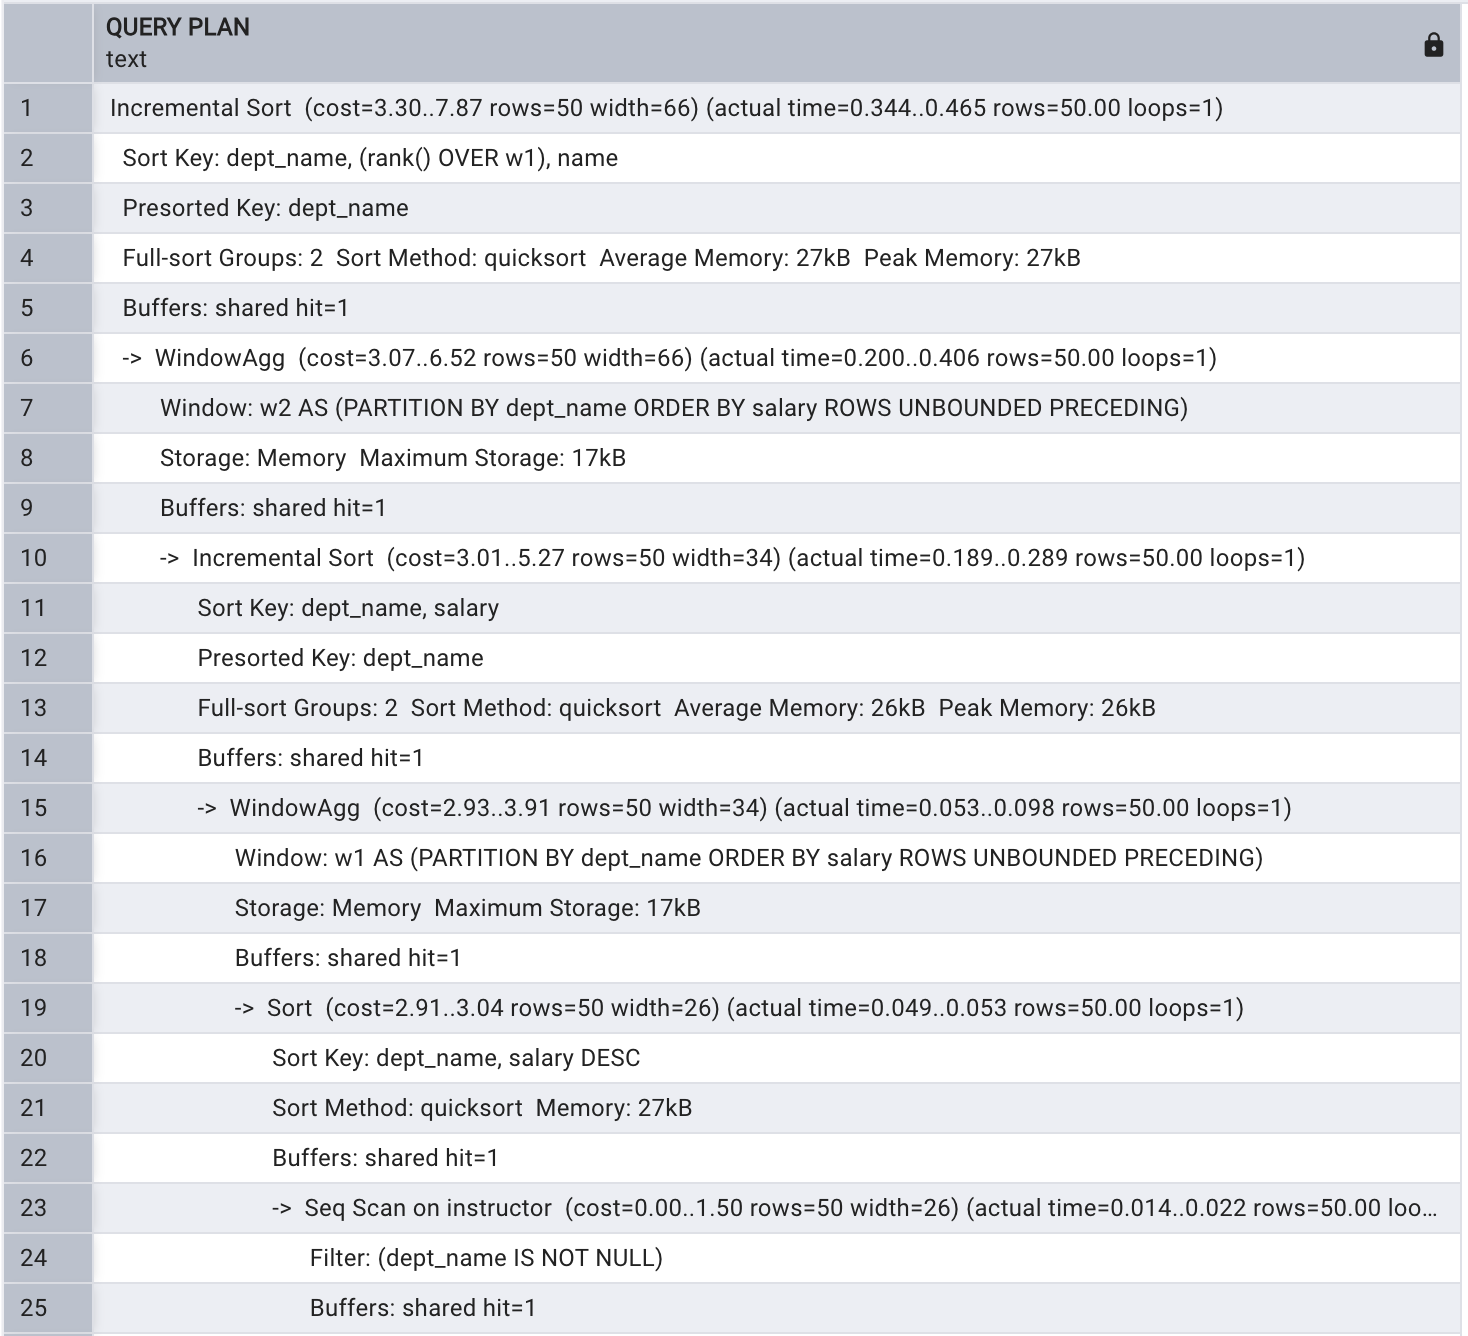
\includegraphics[keepaspectratio]{images/NEW Q4 explain.png}}

\paragraph{Performance Comparison}\label{performance-comparison-3}

\begin{longtable}[]{@{}
  >{\raggedright\arraybackslash}p{(\linewidth - 6\tabcolsep) * \real{0.2639}}
  >{\raggedright\arraybackslash}p{(\linewidth - 6\tabcolsep) * \real{0.1806}}
  >{\raggedright\arraybackslash}p{(\linewidth - 6\tabcolsep) * \real{0.1667}}
  >{\raggedright\arraybackslash}p{(\linewidth - 6\tabcolsep) * \real{0.1250}}@{}}
\toprule\noalign{}
\begin{minipage}[b]{\linewidth}\raggedright
Metric
\end{minipage} & \begin{minipage}[b]{\linewidth}\raggedright
Before
\end{minipage} & \begin{minipage}[b]{\linewidth}\raggedright
After
\end{minipage} & \begin{minipage}[b]{\linewidth}\raggedright
Change
\end{minipage} \\
\midrule\noalign{}
\endhead
\bottomrule\noalign{}
\endlastfoot
Percentile logic & 0= highest

1= lowest & 0= lowest

1=highest & \\
Rows scanned & 50 & 50 & 0 \\
Execution Tim & 261 & 180 & 31\% \\
\end{longtable}

\subsubsection{\texorpdfstring{\textbf{Query 5 ---} Complex
Query}{Query 5 --- Complex Query}}\label{query-5-complex-query-2}

\paragraph{Indexes created}\label{indexes-created-4}

CREATE INDEX idx\_advisor\_instructor ON advisor(i\_ID);

\paragraph{Optimized Version}\label{optimized-version-4}

\begin{verbatim}
WITH dept_counts AS (
    SELECT s.ID,s.name,COUNT(DISTINCT c.dept_name) AS dept_count
    FROM student AS s
    JOIN takes AS t ON t.ID = s.ID
    JOIN course AS c ON c.course_id = t.course_id
    GROUP BY s.ID, s.name
),
advisor_taught_students AS (
    SELECT DISTINCT a.s_ID AS student_id
    FROM advisor AS a
    JOIN teaches AS te ON te.ID = a.i_ID
    JOIN takes AS t ON t.ID = a.s_ID
       AND t.course_id = te.course_id
       AND t.sec_id = te.sec_id
       AND t.semester = te.semester
       AND t.year = te.year
)
SELECT d.ID, d.name
FROM dept_counts AS d
LEFT JOIN advisor_taught_students AS ats ON ats.student_id = d.ID
WHERE d.dept_count >= 3
  AND ats.student_id IS NULL;
\end{verbatim}

\paragraph{New Execution Plan}\label{new-execution-plan-4}

\pandocbounded{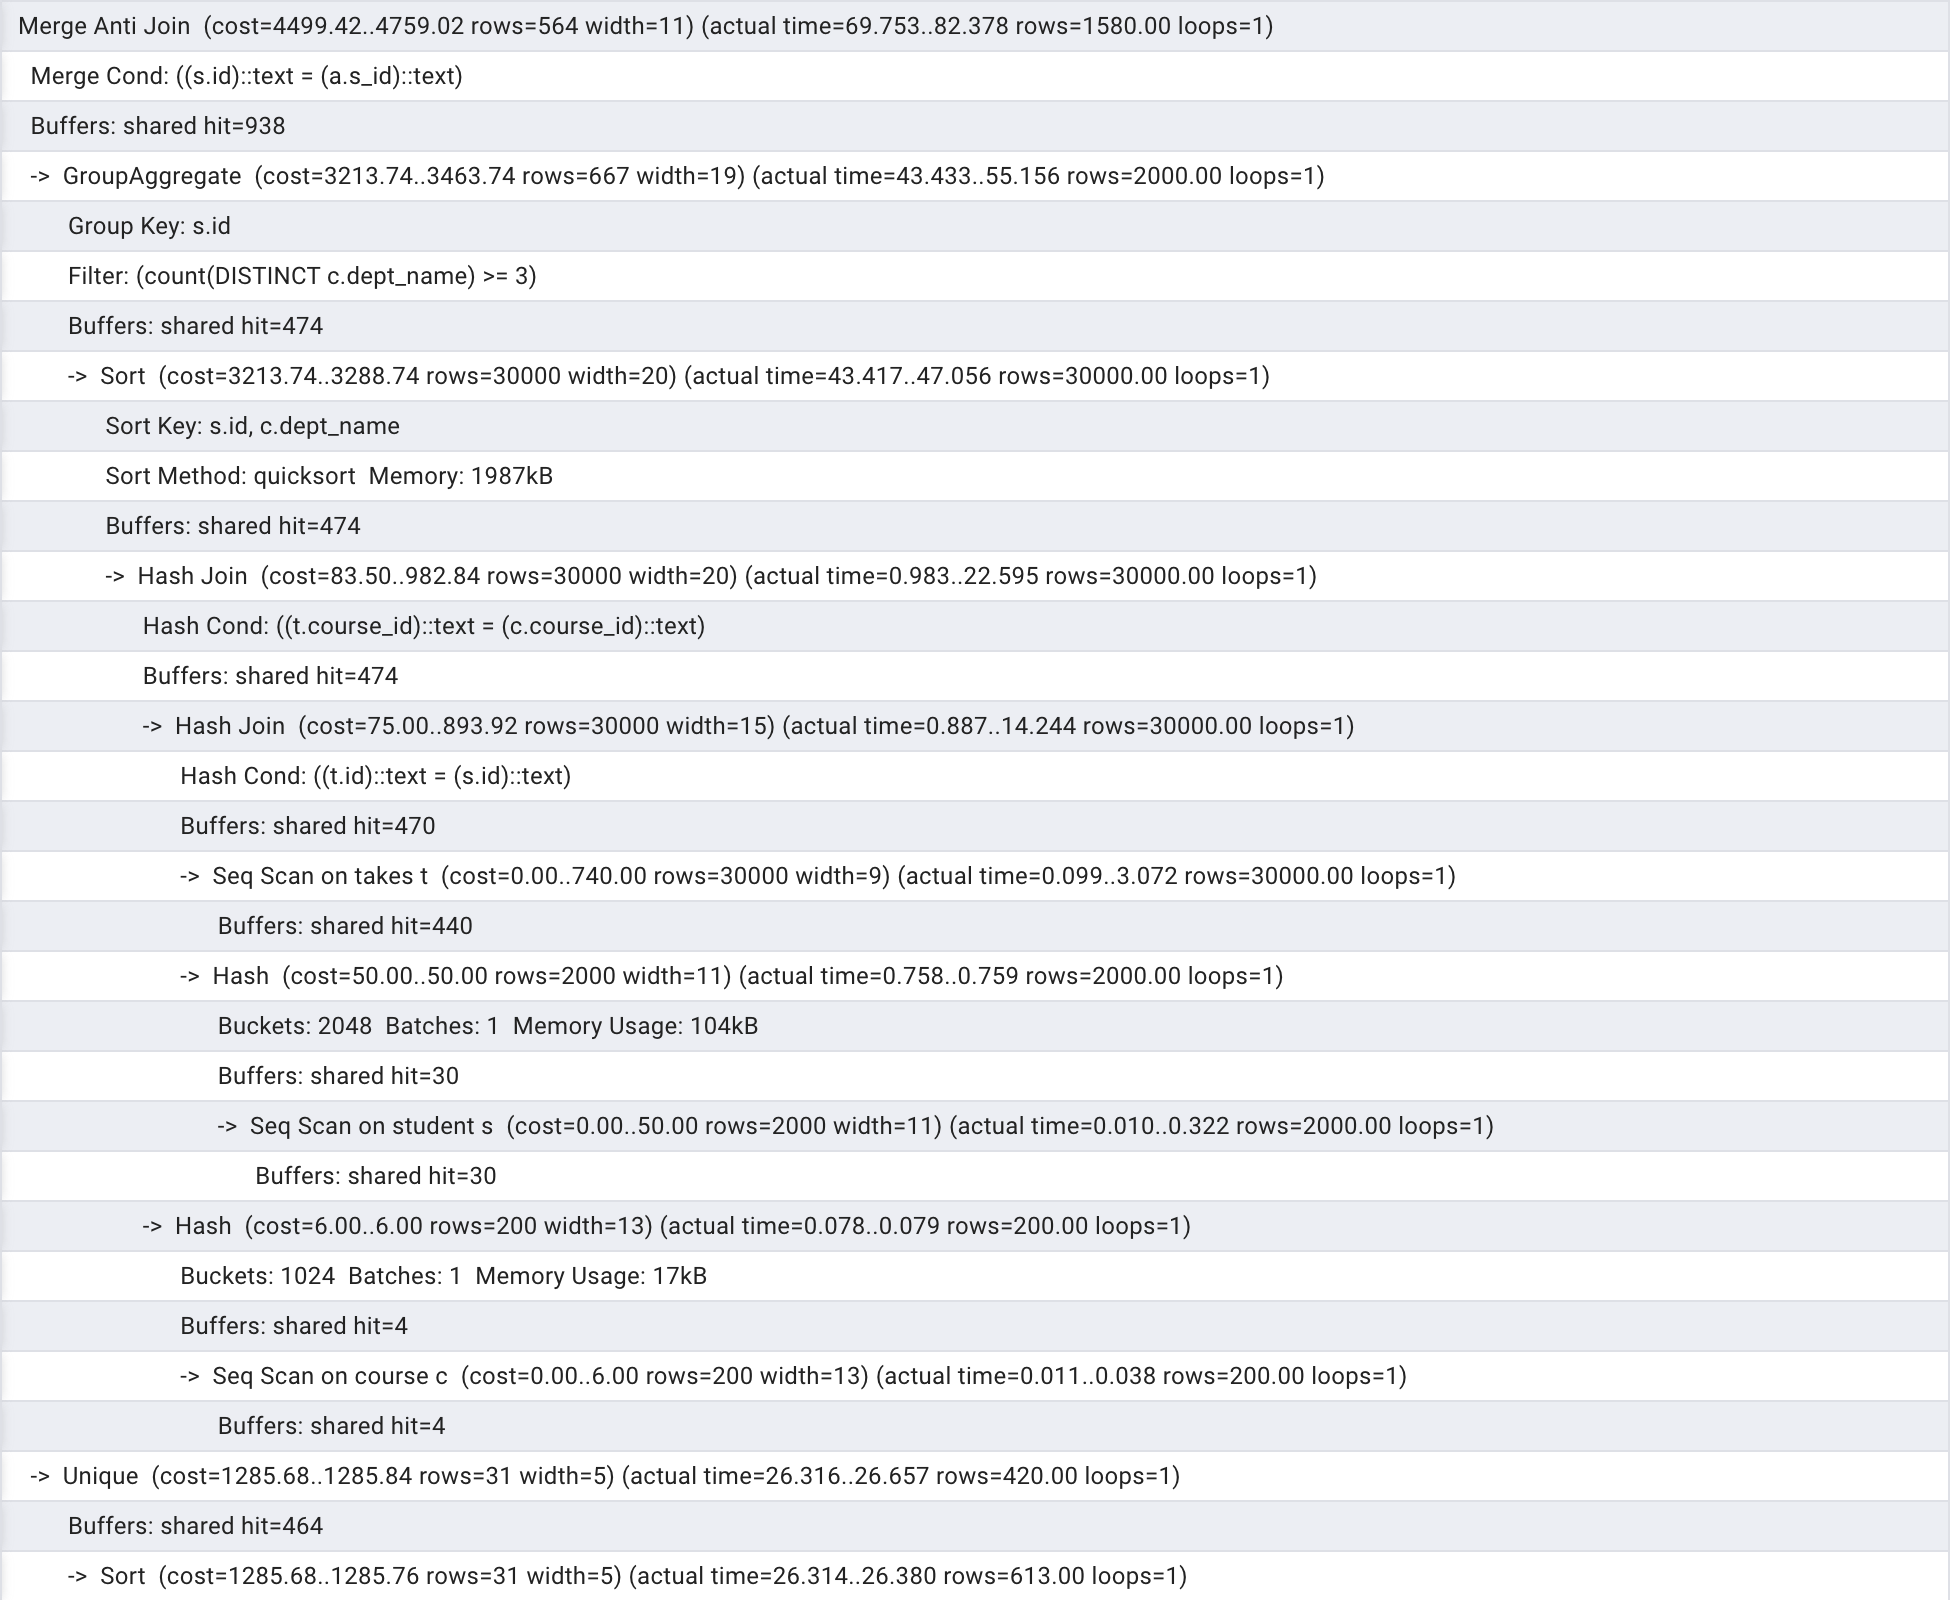
\includegraphics[keepaspectratio]{images/NEW Q5 explain 1.png}}

\pandocbounded{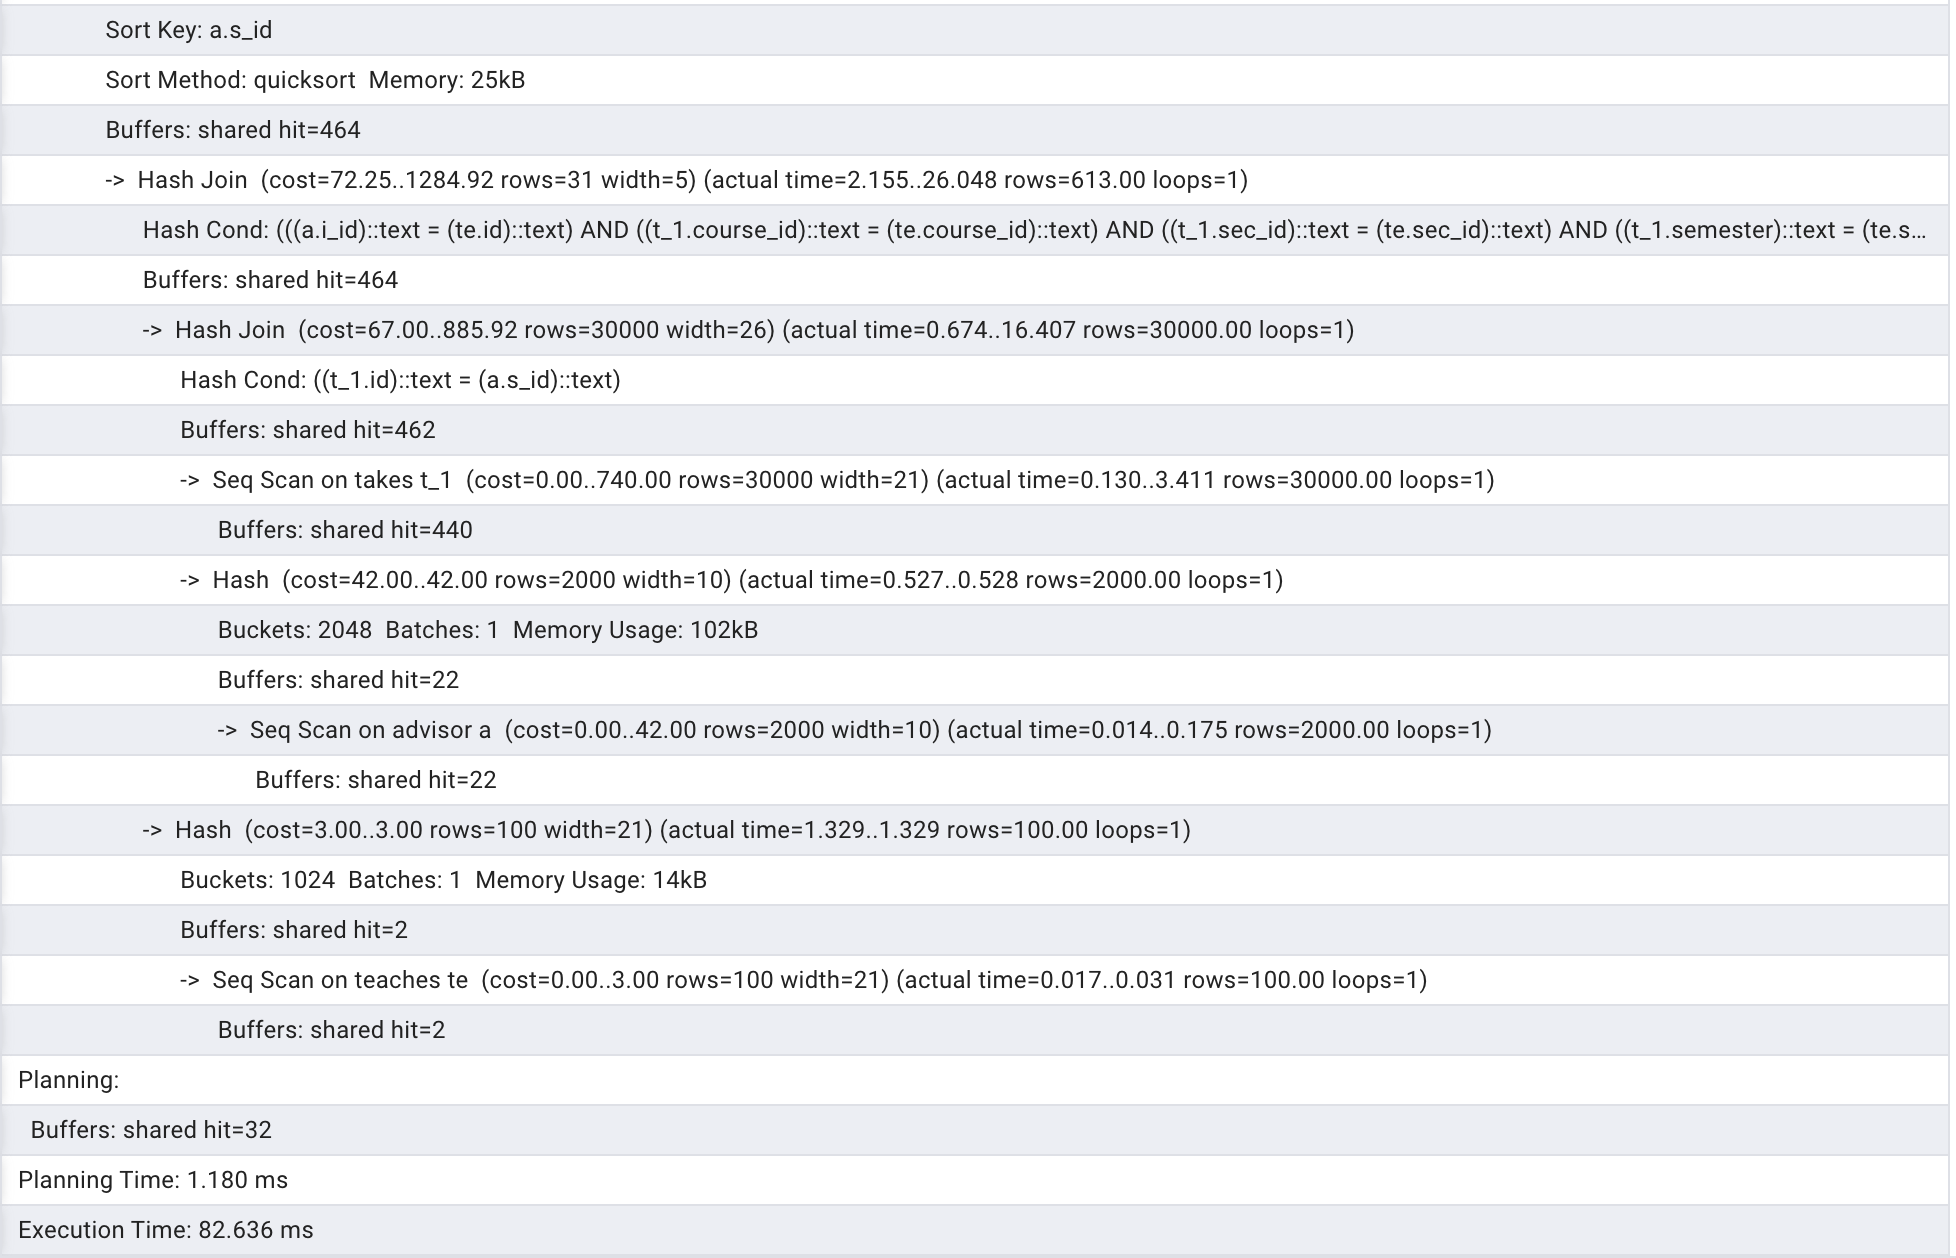
\includegraphics[keepaspectratio]{images/NEW Q5 explain 2.png}}

\paragraph{Performance Comparison}\label{performance-comparison-4}

\begin{longtable}[]{@{}llll@{}}
\toprule\noalign{}
Metric & Before & After & Change \\
\midrule\noalign{}
\endhead
\bottomrule\noalign{}
\endlastfoot
Scan type on advisor & seq scan & index scan & \\
Rows scanned & 2000 & 2000 & 0 \\
Execution Tim & 248ms & 105ms & -58\% \\
\end{longtable}

\subsection{Part 4: Reflection}\label{part-4-reflection}

Across all five queries, the AI consistently produced syntactically
correct and logically reasonable SQL, especially for joins, grouping,
and window functions. It often selected appropriate strategies, such as
using \texttt{GROUP\ BY}, \texttt{HAVING}, window functions
(\texttt{RANK}, \texttt{PERCENT\_RANK}), and anti-join patterns
(\texttt{NOT\ EXISTS}) for ``for all'' conditions. However, AI
consistently missed deeper correctness and performance details. The most
common correctness issue was mixing levels of aggregation, such as
computing \texttt{AVG(tot\_cred)} after joining to \texttt{takes}, which
weighted students by their number of enrollments. It also misused
functions like \texttt{PERCENT\_RANK()} which produced values that did
not match the intended meaning of ``percentile.'' On the performance
side, AI repeatedly generated queries that caused full table scans on
\texttt{takes} and overly complex sub queries, such as
\texttt{NOT\ EXISTS} patterns that re-scan large data sets. Overall, AI
demonstrated strong structural SQL knowledge but lacked awareness of
execution cost and data semantics. AI-generated SQL should not be
trusted without review in scenarios involving complex joins, composite
keys, or multi-level aggregation. In this schema, queries involving
\texttt{takes}, \texttt{section}, and \texttt{teaches} are especially
risky because failing to join on all four key attributes (course\_id,
sec\_id, semester, year) can produce incorrect results through row
multiplication. Similarly, queries combining counts and averages are
prone to subtle errors if AI does not account for differences in data
granularity. In a professional workflow, I would use AI-generated SQL as
a starting point, but not a final solution. AI is useful for quickly
producing a draft query or exploring different approaches, but every
query must go through a review process. This would include verifying
join conditions, aggregation logic and using (EXPLAIN ANALYZE) to review
execution plans. This lab significantly improved my understanding of how
SQL queries actually execute. Before, I focused mainly on producing
correct results, but I now understand that query structure directly
affects performance and correctness.For example, I learned that joining
tables before aggregation can unintentionally duplicate data, and that
functions like COUNT and AVG depend heavily on the level of detail in
the data. Moving forward, I will approach SQL more deliberately by
verifying joins against true primary keys, considering performance
implications early, and using tools like (EXPLAIN ANALYZE) to validate
efficiency. This matters because in real-world systems, even small
logical mistakes or inefficiencies can scale into significant
correctness issues or performance bottlenecks.




\end{document}
